% This is "aamas2010_submissionExample.tex" July 2010
% This file should be compiled with "aamas2010.cls" July 2010
%
% This example file demonstrates the use of the 'aamas2010.cls'
% LaTeX2e document class file. It is for those submitting
% articles to AAMAS 2010 conference. This file is based on
% the sig-alternate.tex example file.
% The 'sig-alternate.cls' file of ACM will produce a similar-looking,
% albeit, 'tighter' paper resulting in, invariably, fewer pages.
% than the original style ACM style.
%
% ----------------------------------------------------------------------------------------------------------------
% This .tex file (and associated .cls ) produces:
%       1) The Permission Statement
%       2) The Conference (location) Info information
%       3) The Copyright Line with AAMAS data
%       4) NO page numbers
%
% as against the acm_proc_article-sp.cls file which
% DOES NOT produce 1) thru' 3) above.
%
% Using 'aamas2010.cls' you don't have control
% from within the source .tex file, over both the CopyrightYear
% (defaulted to 200X) and the IFAAMAS Copyright Data
% (defaulted to X-XXXXX-XX-X/XX/XX).
% These information will be overwritten by fixed AAMAS 2010 information
% in the style files - it is NOT as you are used with ACM style files.
%
% ---------------------------------------------------------------------------------------------------------------
% This .tex source is an example which *does* use
% the .bib file (from which the .bbl file % is produced).
% REMEMBER HOWEVER: After having produced the .bbl file,
% and prior to final submission, you *NEED* to 'insert'
% your .bbl file into your source .tex file so as to provide
% ONE 'self-contained' source file.
%
% This is the document class for full paper submission
\documentclass{aamas2010}

% if you are using PDF LaTex and you cannot find a way for producing
% letter, the following explicit settings may help

\pdfpagewidth=8.5truein
\pdfpageheight=11truein



% Use the postscript times font!
\usepackage{times}

% the following package is optional:
\usepackage{latexsym} 
\usepackage{amsmath}
\usepackage{amssymb}
\usepackage{subfigure}

% Load pfg package for drawing transition systems
\usepackage{xspace}
\usepackage{url}

\usepackage{tikz,pgf}
\usetikzlibrary{arrows,automata,trees,plotmarks,calc}


\usepackage{algorithm}
\usepackage{algorithmic}
%\usepackage[ruled,vlined]{algorithm2e}

\usepackage{textcomp}

% \usepackage[sort&compress,numbers]{natbib}

%% How deep we want to number sections/subsections
\setcounter{secnumdepth}{1}  


% \renewcommand{\baselinestretch}{0.965}

\usepackage{comment}



%%%%%%%%%%%%%%%%%%%%%%%%%%%%%%%%%%%%%%%%%%%%%%%%%%%%%%%%%%%%%%%%%%%%%%%%
%%%%% START OF MACROS
%%%%%%%%%%%%%%%%%%%%%%%%%%%%%%%%%%%%%%%%%%%%%%%%%%%%%%%%%%%%%%%%%%%%%%%%
%%%%%%%%%%%%%%%%%%%%%%%%%%%%%%%%%%%%%%%%%%%%%%%%%%%%
% PERSONAL LaTex MACROS 
%	SEBASTAN SARDINA -- ssardina@cs.rmit.edu.au
%%%%%%%%%%%%%%%%%%%%%%%%%%%%%%%%%%%%%%%%%%%%%%%%%%%%



%%%%%%%%%%%%%%%%%%%%%%%%%%%%%%%%%%%%%%%%%%%%%%%%%%%%
% Font modes & definitions
%%%%%%%%%%%%%%%%%%%%%%%%%%%%%%%%%%%%%%%%%%%%%%%%%%%%

% conditional math environment
% \gdef\Math#1{\ifmmode #1 \else \mbox{$#1$}\fi}
\newcommand{\Math}[1]{\ensuremath{#1}}



\newcommand{\modesf}[1]{{\Math{\mathsf{#1}}}}
\newcommand{\modecal}[1]{{\Math{\mathcal{#1}}}}
\newcommand{\modeit}[1]{{\Math{\mathit{#1}}}}


\newcommand{\textmath}[1]{{\mbox{\textit{#1}}}}


%%%%%%%%%%%%%%%%%%%%%%%%%%%%%%%%%%%%%%%%%%%%%%%%%%%%
% Proper names
%%%%%%%%%%%%%%%%%%%%%%%%%%%%%%%%%%%%%%%%%%%%%%%%%%%%
\newcommand{\propername}[1]{\mbox{\small \textsf{#1}}}

\newcommand{\Golog}{\propername{Golog}}
\newcommand{\GologSpeak}{\propername{GologSpeak}}
\newcommand{\DGolog}{\propername{DGolog}}
\newcommand{\sGolog}{\propername{sGolog}}
\newcommand{\ConGolog}{\propername{ConGolog}}
\newcommand{\IndiGolog}{\propername{IndiGolog}}
\newcommand{\LeGolog}{\propername{LeGolog}}
\newcommand{\DTGolog}{\propername{DTGolog}}
\newcommand{\Prolog}{\propername{Prolog}}
\newcommand{\AgentSpeak}{\propername{AgentSpeak}}
\newcommand{\JASON}{\propername{Jason}}
\newcommand{\CANMINUS}{\propername{\CAN$^{\A}$}}
\newcommand{\CANMINUST}{\propernametiny{Can$^{\cal C}$}}
\newcommand{\CAN}{\propername{CAN}}
\newcommand{\CANT}{\propernametiny{Can}}
\newcommand{\CANPLAN}{\propername{CANPlan}}
\newcommand{\CANPLANT}{\propernametiny{CanPlan}}
\newcommand{\CANPLANII}{\propername{CanPlan2}}
\newcommand{\CANPLANOR}{\propername{Can(Plan)}}
\newcommand{\CANGOAL}{\propername{CanGoal}}
\newcommand{\JACK}{\propername{Jack}}
\newcommand{\JACKTM}{\propername{Jack\texttrademark}}
\newcommand{\JAM}{\propername{JAM}}
\newcommand{\PRS}{\propername{PRS}}
\newcommand{\SPARK}{\propername{SPARK}}
\newcommand{\RAP}{\propername{Rap}}
\newcommand{\dMARS}{\propername{dMARS}}
\newcommand{\TAPL}{\propername{3APL}}
\newcommand{\DAPL}{\propername{2APL}}
\newcommand{\GOALBDI}{\propername{GOAL}}
\newcommand{\JSHOP}{\propername{JSHOP}}
\newcommand{\JSHOPII}{\propername{JSHOP2}}
\newcommand{\ASHOP}{\propername{A-SHOP}}
\newcommand{\SHOP}{\propername{SHOP}}
\newcommand{\SHOPII}{\propername{SHOP2}}
\newcommand{\ACT}{\propername{ACT}}
\newcommand{\SIPEII}{\propername{SIPE-2}}
\newcommand{\OPLANII}{\propername{O-PLAN2}}
\newcommand{\Retsina}{\propername{Retsina}}
\newcommand{\IPEM}{\propername{IPEM}}
\newcommand{\SAGE}{\propername{Sage}}
\newcommand{\DECAF}{\propername{Decaf}}
\newcommand{\PROPICE}{\propername{Propice-Plan}}
\newcommand{\CYPRESS}{\propername{Cypress}}
\newcommand{\CPEF}{\propername{CPEF}}
\newcommand{\JADEX}{\propername{JADEX}}
\newcommand{\IMPACT}{\propername{IMPACT}}
\newcommand{\PDT}{\propername{PDT}}


%%%%%%%%%%%%%%%%%%%%%%%%%%%%%%%%%%%%%%%%%%%%%%%%%%%%
% Calligraphic letters - Taken from Giuseppe De Giacomo 2006
%%%%%%%%%%%%%%%%%%%%%%%%%%%%%%%%%%%%%%%%%%%%%%%%%%%%
\newcommand{\A}{\modecal{A}} \newcommand{\B}{\modecal{B}}
\newcommand{\C}{\modecal{C}} \newcommand{\D}{\modecal{D}}
\newcommand{\E}{\modecal{E}} \newcommand{\F}{\modecal{F}}
\newcommand{\G}{\modecal{G}} \renewcommand{\H}{\modecal{H}}
\newcommand{\I}{\modecal{I}} \newcommand{\J}{\modecal{J}}
\newcommand{\K}{\modecal{K}} \renewcommand{\L}{\modecal{L}}
\newcommand{\M}{\modecal{M}} \newcommand{\N}{\modecal{N}}
\renewcommand{\O}{\modecal{O}} \renewcommand{\P}{\modecal{P}}
\renewcommand{\S}{\modecal{S}} \newcommand{\T}{\modecal{T}}
\newcommand{\U}{\modecal{U}} \newcommand{\V}{\modecal{V}}
\newcommand{\W}{\modecal{W}} \newcommand{\X}{\modecal{X}}
\newcommand{\Y}{\modecal{Y}} \newcommand{\Z}{\modecal{Z}}
\newcommand{\R}{\modecal{R}} 



%%%%%%%%%%%%%%%%%%%%%%%%%%%%%%%%%%%%%%%%%%%%%%%%%%%%
% Situation Calculus macros
%%%%%%%%%%%%%%%%%%%%%%%%%%%%%%%%%%%%%%%%%%%%%%%%%%%%

% Sitcalc Golog/ConGolog/IndiGolog programs
\newcommand{\mif}{\mbox{\bf if}}
\newcommand{\mwhile}{\mbox{\bf while}}
\newcommand{\mreturn}{\mbox{\bf return}}
\newcommand{\mthen}{\mbox{\bf then}}
\newcommand{\melse}{\mbox{\bf else}}
\newcommand{\mdo}{\mbox{\bf do}}
\newcommand{\mnoOp}{\mbox{\bf $noOp$}}
\newcommand{\mproc}{\mbox{\bf proc}}
\newcommand{\mend}{\mbox{\bf end}}
\newcommand{\mendproc}{\mbox{\bf endProc}}
\newcommand{\mendif}{\mbox{\bf endIf}}
\newcommand{\mendwhile}{\mbox{\bf endWhile}}
\newcommand{\mendfor}{\mbox{\bf endFor}}
\newcommand{\mfor}{\mbox{\bf for}}
\def\prparallel{\mathrel{\rangle\!\rangle}}
\def\supparallel{\mathord{|\!|}}
\newcommand{\conc}{\mbox{$\parallel$}}
\newcommand{\pconc}{\mbox{$\prparallel$}}
\newcommand{\search}{\mbox{$\Sigma$}}
\newcommand{\searchO}{\mbox{$\Sigma_o$}}
\newcommand{\searchOM}{\mbox{$\Sigma_o^M$}}
\newcommand{\searchCR}{\mbox{$\Sigma_{cr}$}}
\newcommand{\searchR}{\mbox{$\Sigma_{r}$}}
\newcommand{\searchM}{\mbox{$\Sigma^M$}}
\newcommand{\searchC}{\mbox{$\Sigma_c$}}
\newcommand{\searchCM}{\mbox{$\searchC^M$}}
\newcommand{\searchCB}{\mbox{$\Sigma_{cb}$}}
\newcommand{\searchD}{\mbox{$\Delta$}}
\newcommand{\searchE}{\mbox{$\Delta_e$}}
\newcommand{\searchEM}{\mbox{$\Delta_e^M$}}
\newcommand{\searchL}{\mbox{$\Delta_l$}}
\newcommand{\searchER}{\mbox{$\Delta_r$}}
\newcommand{\searchERM}{\mbox{$\Delta_r^M$}}
\newcommand{\mnt}{\mbox{$mnt$}}


%%% Knowledge in sitcalc
\newcommand{\Know}{\mbox{\bf Know}}
\newcommand{\KWhether}{\mbox{\bf KWhether}}
\newcommand{\Kref}{\mbox{\bf KRef}}
\newcommand{\nows}{{\hbox{\small\sf now}}}
\newcommand{\now}{{\mbox{\sf now}}}


% IndiGolog macros
\newcommand{\Sensed}{\textmath{Sensed}}
\newcommand{\hend}{\textmath{end}}
\newcommand{\Trans}{\textmath{Trans}}
\newcommand{\Final}{\textmath{Final}}
\newcommand{\Poss}{\textmath{Poss}}
\newcommand{\Transobs}{\textmath{TransObs}}


%%%%%%%%%%%%%%%%%%%%%%%%%%%%%%%%%%%%%%%%%%%%%%%%%%%%
% CAN notation for BDI Agents
%%%%%%%%%%%%%%%%%%%%%%%%%%%%%%%%%%%%%%%%%%%%%%%%%%%%
\newcommand{\Goal}{\modesf{Goal}}
\newcommand{\GoalS}{\modesf{G}}
\newcommand{\SGoal}{\modesf{SGoal}}
\newcommand{\SGoalS}{\modesf{SG}}
\newcommand{\goal}[3]{{\sf Goal}(#1,#3,#2)}
\newcommand{\goalp}[3]{{\sf Goal}_{P}(#1,#3,#2)}
\newcommand{\goalsfp}{\goal{s}{f}{P}}
\newcommand{\goalsfpp}{\goalp{s}{f}{P}}
\newcommand{\goalt}[2]{{\sf Goal}(#1,#2)}
\newcommand{\goalsf}{\goal{s}{f}}

\newcommand{\Plan}{\modesf{Plan}}
\newcommand{\PlanP}{\modesf{P}}
\newcommand{\PlanArg}[1]{\Plan(#1)}

\newcommand{\pnil}{\mbox{\textit{nil}}}
\newcommand{\ptrue}{\mbox{\textit{true}}}
\newcommand{\pfalse}{\mbox{\textit{false}}}
\newcommand{\pfail}{\mbox{\textit{fail}}}

\newcommand{\pguardaltl}[1]{\mbox{$\altl #1 \altr$}} % guarded alternatives
\newcommand{\altl}{\llparenthesis}
\newcommand{\altr}{\rrparenthesis}

%% Macro for BDI plan rules:  \plane{a:b<-c} \plans{a<-c}
\newcommand\plane[1]{\planeaux!#1!}
\def\planeaux!#1:#2<-#3!{\Math{#1 \mbox{\rm:} #2\; \leftarrow #3}}
\newcommand\plans[1]{\planeaux!#1!}
\def\planeaux!#1<-#2!{\Math{#1 \leftarrow #2}}




%%%%%%%%%%%%%%%%%%%%%%%%%%%%%%%%%%%%%%%%%%%%%%%%%%%%
% START - Operational semantics
%%%%%%%%%%%%%%%%%%%%%%%%%%%%%%%%%%%%%%%%%%%%%%%%%%%%
% Labels
\newcommand{\bdi}{bdi}
\newcommand{\htn}{plan}
\newcommand{\transitionlabel}[1]{\modesf{{#1}}}

% Meta-transition
\newcommand{\mtransition}{\Longrightarrow} % meta transition
\newcommand{\mtransitionstar}{\overset{*}{\mtransition}} % trans meta closure
\newcommand{\mtransitiontype}[1]{\overset{\transitionlabel{#1}}{\mtransition}}
\newcommand{\mtransitionstartype}[1]{\overset{*}{\mtransitiontype{#1}}}

% Transition
\newcommand{\transition}{\longrightarrow} 	% regular transition

\newcommand{\transitionstar}{\overset{*}{\transition}} % trans closure
\newcommand{\transitionst}{\overset{*}{\transition}} %trans closure
\newcommand{\transitionanot}[1]{\transition_{#1}} 	% regular transition
\newcommand{\transitionbdistarint}
	{\overset{\transitionlabel{\bdi}_{*}}{\transition_i}}

\newcommand{\transitiontype}[1]{\overset{\transitionlabel{#1}}{\transition}}
\newcommand{\transitionbdi}{\overset{\transitionlabel{\bdi}}{\transition}}
\newcommand{\transitionhtn}{\overset{\transitionlabel{\htn}}{\transition}}
\newcommand{\transitionhtnstar}
	{\overset{\transitionlabel{\htn}_{*}}{\transition}}
\newcommand{\transitionbdistar}
{\overset{\transitionlabel{\bdi}_{*}}{\transition}}

\newcommand{\transitionhtnk}[1]
{\overset{\transitionlabel{\htn}_{#1}}{\transition}}
\newcommand{\transitionbdik}[1]
{\overset{\transitionlabel{\bdi}_{#1}}{\transition}}



%%%%%%%%%%%%%%%%%%%%%%%%%%%%%%%%%%%%%%%%%%%%%%%%%%%%
% Several notations
%%%%%%%%%%%%%%%%%%%%%%%%%%%%%%%%%%%%%%%%%%%%%%%%%%%%

%%%%%%%%%%%%%%%%%%%%%%%%%% Delimiters
\newcommand{\quotes}[1]{{\lq\lq #1\rq\rq}}
\newcommand{\set}[1]{\{#1\}}                      % set
\newcommand{\Set}[1]{\left\{#1\right\}}
\newcommand{\bigmid}{\Big|}
\newcommand{\card}[1]{|{#1}|}                     % cardinality of a set
\newcommand{\Card}[1]{\left| #1\right|}
\newcommand{\cards}[1]{\sharp #1}
\newcommand{\sub}[1]{[#1]}
\newcommand{\tuple}[1]{\Math{\langle #1 \rangle}}		% tuple
\newcommand{\Tuple}[1]{\Math{\left\langle #1 \right\rangle}}		% tuple
\newcommand{\tup}[1]{\tuple{#1}}            			% tuple
\newcommand{\Tup}[1]{\Tuple{#1}}
\newcommand{\config}[1]{\tuple{#1}}	% configuration

% A symbol with something on top and under: \underoverset{under}{above}{text}
\newcommand{\underoverset}[3]{\underset{#1}{\overset{#2}{#3}}}


\newcommand{\myi}{\emph{(i)}\xspace}
\newcommand{\myii}{\emph{(ii)}\xspace}
\newcommand{\myiii}{\emph{(iii)}\xspace}
\newcommand{\myiv}{\emph{(iv)}\xspace}
\newcommand{\myv}{\emph{(v)}\xspace}
\newcommand{\myvi}{\emph{(vi)}\xspace}


%%%%%%%%%%%%%%%%%%%%%%%%%%%%%%%%%%%%%%%%%%%%%%%%%%%%
% Several useful symbols
%%%%%%%%%%%%%%%%%%%%%%%%%%%%%%%%%%%%%%%%%%%%%%%%%%%%

% Symbols
\newcommand{\powerset}{\mathbb{P}}
\newcommand{\NatN}{\Math{\mathbb{N}_0}} % naturals+0
\newcommand{\Nat}{\Math{\mathbb{N}}}
\newcommand{\mgu}{\modesf{mgu}}
\newcommand{\complexsub}{\modesf{cplex}}

% True and False
\newcommand{\true}{\mathtt{true}}
\newcommand{\false}{\mathtt{false}}
\newcommand{\True}{\mathtt{True}}
\newcommand{\False}{\mathtt{False}}
\newcommand{\TRUE}{\uppercase{\true}}
\newcommand{\FALSE}{\uppercase{\false}}

% LTL modalities
\newcommand{\mnext}{\bigcirc}		% next
\newcommand{\malways}{\square}		% always
\newcommand{\meventually}{\lozenge}	% eventually
\newcommand{\muntil}{\mathop{\U}}	% until

% Relations
\newcommand{\goto}[1]{\stackrel{#1}{\longrightarrow}}
\newcommand{\gotoii}[2]{\underoverset{#2}{#1}{\longrightarrow}}
\newcommand{\isdef}{\hbox{$\stackrel{\mbox{\tiny def}}{=}$}}

%%%%%%%%%%%%%%%%%%%%%%%%%%%%%%%%%%%%%%%%%%%%%%%%%%%%
% Macros for Proofs
%%%%%%%%%%%%%%%%%%%%%%%%%%%%%%%%%%%%%%%%%%%%%%%%%%%%

% Proofs symbols: provided by amsmath package now as \qed
\newcommand{\qedblack}{\phantom{a} \hfill \ensuremath{\blacksquare}}



\long\def\eatpar#1{%
\ifx#1\par                      % se il token e' \par
\let\nextmove=\eatpar           % rimetti \eatpar in coda
\else
\let\nextmove=#1%               altrimenti, rimetti il token in coda
\fi
\nextmove%                      il token o \eatpar viene rimesso in coda
}

\def\qed{\hfill{\qedboxempty}      % qed with empty box
  \ifdim\lastskip<\medskipamount \removelastskip\penalty55\medskip\fi}

\def\qedboxempty{\vbox{\hrule\hbox{\vrule\kern3pt
                 \vbox{\kern3pt\kern3pt}\kern3pt\vrule}\hrule}}

\def\qedfull{\hfill{\qedboxfull}   % qed with full box
  \ifdim\lastskip<\medskipamount \removelastskip\penalty55\medskip\fi}

\def\qedboxfull{\vrule height 4pt width 4pt depth 0pt}

\newcommand{\markfull}{\qedfull}
\newcommand{\markempty}{\qed}


%%%%%%%%%%%%%%%%%%%%%%%%%%%%%%%%%%%%%%%%%%%%%%%%%%%%
% Several special text abbreviations
%%%%%%%%%%%%%%%%%%%%%%%%%%%%%%%%%%%%%%%%%%%%%%%%%%%%

% Italic-text abbreviations (sets, etc.)
\newcommand{\CNF}{\modeit{CNF}}
\newcommand{\Actions}{\modeit{Act}}
\newcommand{\Events}{\modeit{Event}}
\newcommand{\freeVar}{\modeit{dom}}
\newcommand{\variant}{\modesf{ren}}
\newcommand{\Init}{\modeit{Init}}

\newcommand{\dummytask}{\mbox{\textit{dummyTask}}}


\newcommand{\BDI}{\mbox{BDI}}

\newcommand{\Active}{\modeit{Act}}






%%%%%%%%%%%%%%%%%%%%%%%%%%%%%%%%%%%%%%%%%%%%%%%%%%%%
% Margin notes for comments  
%%%%%%%%%%%%%%%%%%%%%%%%%%%%%%%%%%%%%%%%%%%%%%%%%%%%
\setlength{\marginparwidth}{0.8in}
\let\oldmarginpar\marginpar
\renewcommand\marginpar[1]{\-\oldmarginpar[\raggedleft\footnotesize #1]%
{\raggedright\footnotesize #1}}

% \setlength{\marginparwidth}{0.5in}
\newcommand{\notem}[1]{\marginpar{\textbf{#1}}}
\newcommand{\notetext}[1]{\notem{OBS} \textit{#1}}

\newcommand{\ncheck}{\notem{CHECK!}}
\newcommand{\GGG}{\notem{GGG}}
\newcommand{\SSS}{\notem{SSS}}
\newcommand{\LIN}{\notem{LP}}
\newcommand{\YVES}{\notem{YL}}




%%%%%%%%%%%%%%%%%%%%%%%%%%%%%%%%%%%%%%%%%%%%%%%%%%%%
% PhD boxed notes for the committee in Toronto -- Taken from Ron Petrick 2004
%%%%%%%%%%%%%%%%%%%%%%%%%%%%%%%%%%%%%%%%%%%%%%%%%%%%
% \usepackage{color}
\newcounter{countphdnote}
% \newcommand{\phdnote}[1]{\textbf{#1}}
% \newcommand{\phdnote}[1]{
% \begin{center}
% \begin{tabular}{c}
% 	\begin{minipage}{4in}
% 		\fcolorbox{black}{black}{\textcolor
%     		{white}{\textbf{\ Note \thecountphdnote\ }}}
% 	\end{minipage} \\
%     	\fcolorbox{black}{white}{
% 	\begin{minipage}{6in}
% 		#1\addtocounter{countphdnote}{1}%
%     	\end{minipage}}
% \end{tabular}
% \end{center}}



%%%%%%%%%%%%%%%%%%%%%%%%%%%%%%%%%%%%%%%%%%%%%%%%%%%%
% Tighter lists -- From Lin Padgham 2007
%%%%%%%%%%%%%%%%%%%%%%%%%%%%%%%%%%%%%%%%%%%%%%%%%%%%
\newcounter{bean}

\newenvironment{tightenumerate}{
                \begin{list}{
                  {\mbox {
                      \arabic{bean}.\/}}}{\usecounter{bean}
                      \setlength{\itemsep}{-1pt}\setlength{\topsep}{0pt}}}{
                \end{list}}

\newenvironment{tightitemize}{
                \begin{list}{$\bullet$}{
                    \setlength{\itemsep}{-1pt}}{\setlength{\topsep}{0pt}}}{
                \end{list}}
%\setlength{\itemsep}{0pt}}{\setlength{\topsep}{0pt}}}{

\renewenvironment{tightenumerate}{\begin{enumerate}}{\end{enumerate}}
\renewenvironment{tightitemize}{\begin{itemize}}{\end{itemize}}




%%%%%%%%%%%%%%%%%%%%%%%%%%%%%%%%%%%%%%%%%%%%%%%%%%%%
% General useful macros
%%%%%%%%%%%%%%%%%%%%%%%%%%%%%%%%%%%%%%%%%%%%%%%%%%%%

% Produces citations as follows: Author (Year)
\newcommand{\citeby}[1]{\citeauthor{#1} (\citeyear{#1})}

% Mark pages (pp. xxx)
\newcommand{\page}{pp.}

% Marker text
\newcommand{\marker}[1]{\textbf{******* \today: #1 *******}}

% Good underline --- Ttaken from Hector Levesque 2003
%	underline with space between text and line
\newcommand{\under}[1]{\mbox{\underline{\it\smash{#1}\vphantom{\lower.05ex\hbox{
x}}}}}

% \newcommand{\defterm}[1]{\under{\textit{#1}}}
\newcommand{\defterm}[1]{\textit{#1}}

% Comments -- just ignore everything: same as \comment{} in comment package
\newcommand{\commentarea}[1]{}

% Finish a page compactly (remove trailing space)
\newcommand{\finishpage}{ \newpage{ \pagestyle{empty} } }

% Separation for itemizations
\newcommand{\separation}[1]{\addtolength{\itemsep}{#1}}




%%%%%%%%%%%%%%%%%%%%%%%%%%%%%%%%%%%%%%%%%%%%%%%%%%%%
% Definition of Environments
%%%%%%%%%%%%%%%%%%%%%%%%%%%%%%%%%%%%%%%%%%%%%%%%%%%%

\newcommand{\finishproof}{\phantom{aaa} \hfill\ }

\newenvironment{myproof}[2]
	{\noindent {\sc Proof of #1 \ref{#2}} (\page\ \pageref{#2}):}
	{ \ \hfill \qed}

% \newenvironment{proof}
% 	{ \normalfont \noindent {\sc Proof:}}
% 	{ \qed}

% \newenvironment{proof}{\begin{proof}}{\begin{end}}
% \newtheorem{proof}{proof}
% \newenvironment{proof}[0]{\textsc{Proof.\ }\normalfont}{\qedsymbol}
\newenvironment{proofsk}{\textsc{Proof (sketch).\ }}{\qed}

% Environments
% \newtheorem{subtheorem}{Theorem}[subsection]
% \newtheorem{theorem}{Theorem}[section]
% \newtheorem{conjecture}[theorem]{Conjecture}
% \newtheorem{corollary}[theorem]{Corollary}
% \newtheorem{definition}[theorem]{Definition}
% \newtheorem{proposition}[theorem]{Proposition}
% \newtheorem{lemma}[theorem]{Lemma}
% \newtheorem{example}[theorem]{Example}
% 
% \newcommand{\Theorem}[1]{ \begin{theorem} #1 \end{theorem} }
% \newcommand{\Definition}[1]{ \begin{definition} #1 \end{definition} }
% \newcommand{\Lemma}[1]{ \begin{lemma} #1 \end{lemma} }
% \newcommand{\Claim}[1]{ \begin{claim} #1 \end{claim} }
% \newcommand{\Example}[1]{ \begin{example} #1 \end{example} }






%%%%%%%%%%%%%%%%%%%%%%%%%%%%%%%%%%%%%%%%%%%%%%%%%%%%
% EOF: macros-sebastian.tex
%%%%%%%%%%%%%%%%%%%%%%%%%%%%%%%%%%%%%%%%%%%%%%%%%%%%

\renewcommand{\defterm}[1]{\under{\textit{#1}}}
\newcommand{\obs}[1]{\notetext{#1}}


\newtheorem{definition}{Definition}
\newtheorem{theorem}{Theorem}
\newtheorem{corollary}{Corollary}
\newtheorem{proposition}{Proposition}
\newtheorem{lemma}{Lemma}
%\newenvironment{proof}{\textsl{Proof.\ }}{$\Box$}
%%\renewenvironment{proof}{\textsl{Proof.\ }}{\qed}
\renewenvironment{proofsk}{\textsl{Proof (sketch).\ }}{$\Box$}



\newcommand{\BUL}{\textsf{\small BUL}}
\newcommand{\CL}{\textsf{\small ACL}}
\newcommand{\dt}{{decision tree}}
\newcommand{\DT}{{Decision Tree}}
\newcommand{\CLSELA}{\mbox{$\CL\!\!+\!\!\Omega$}}
\newcommand{\CLSELB}{\mbox{$\CL\!\!+\!\!\Omega'$}}
\newcommand{\BULSELA}{\mbox{$\BUL\!\!+\!\!\Omega$}}
\newcommand{\BULSELB}{\mbox{$\BUL\!\!+\!\!\Omega'$}}



%%%%%%%%%%%%%%%%%%%%%%%%%%%%%%%%%%%%%%%%%%%%%%%%%%%%%%%%%%%%%%%%%%%%%%%%
%%%%% END OF MACROS
%%%%%%%%%%%%%%%%%%%%%%%%%%%%%%%%%%%%%%%%%%%%%%%%%%%%%%%%%%%%%%%%%%%%%%%%



%%% STYLES FOR THE PICTURES
\tikzstyle{every initial by arrow}=[initial text=]
% \tikzstyle{every state}=[fill=none,draw=black,text=black]
\tikzstyle{every state}=[fill=none,draw=black,text=black,inner sep=0pt,minimum
size=7mm]
\tikzstyle{every picture}=[->,>=stealth',shorten >=1pt,auto,node distance=2.5cm,
semithick]
\tikzstyle{sim}=[->,dotted]




\newcommand{\Omit}[1]{}

\begin{document}

% In the original styles from ACM, you would have needed to
% add meta-info here. This is not necessary for AAMAS 2010 as
% the complete copyright information is generated by the cls-files.

% For appropriate information about authors and title written in the
% copyright information, you must use these commands. Note that the copyright
% box is not required for the initial submission.

\AuthorsForCitationInfo{All Authors}

\TitleForCitationInfo{Learning Context Conditions for BDI Plan Selection}

\title{Learning Context Conditions for BDI Plan Selection}

% AUTHORS
\author{Tracking Number: 170}

% For initial submission, do not give author names, but the
% tracking number, instead, as the review process is blind.

% You need the command \numberofauthors to handle the 'placement
% and alignment' of the authors beneath the title.
%
% For aesthetic reasons, we recommend 'three authors at a time'
% i.e. three 'name/affiliation blocks' be placed beneath the title.
%
% NOTE: You are NOT restricted in how many 'rows' of
% "name/affiliations" may appear. We just ask that you restrict
% the number of 'columns' to three.
%
% Because of the available 'opening page real-estate'
% we ask you to refrain from putting more than six authors
% (two rows with three columns) beneath the article title.
% More than six makes the first-page appear very cluttered indeed.
%
% Use the \alignauthor commands to handle the names
% and affiliations for an 'aesthetic maximum' of six authors.
% Add names, affiliations, addresses for
% the seventh etc. author(s) as the argument for the
% \additionalauthors command.
% These 'additional authors' will be output/set for you
% without further effort on your part as the last section in
% the body of your article BEFORE References or any Appendices.

%\numberofauthors{8} %  in this sample file, there are a *total*
% of EIGHT authors. SIX appear on the 'first-page' (for formatting
% reasons) and the remaining two appear in the \additionalauthors section.
%

%\author{

% You can go ahead and credit any number of authors here,
% e.g. one 'row of three' or two rows (consisting of one row of three
% and a second row of one, two or three).
%
% The command \alignauthor (no curly braces needed) should
% precede each author name, affiliation/snail-mail address and
% e-mail address. Additionally, tag each line of
% affiliation/address with \affaddr, and tag the
% e-mail address with \email.

% 1st. author
%\alignauthor
%Ben Trovato\titlenote{Dr.~Trovato insisted his name be first.}\\
%       \affaddr{Institute for Clarity in Documentation}\\
%       \affaddr{1932 Wallamaloo Lane}\\
%       \affaddr{Wallamaloo, New Zealand}\\
%       \email{trovato@corporation.com}

% 2nd. author
%\alignauthor
%G.K.M. Tobin\titlenote{The secretary disavows
%any knowledge of this author's actions.}\\
%       \affaddr{Institute for Clarity in Documentation}\\
%       \affaddr{P.O. Box 1212}\\
%       \affaddr{Dublin, Ohio 43017-6221}\\
%       \email{webmaster@marysville-ohio.com}

% 3rd. author
%\alignauthor Lars Th{\o}rv{\"a}ld\titlenote{This author is the
%one who did all the really hard work.}\\
%       \affaddr{The Th{\o}rv{\"a}ld Group}\\
%       \affaddr{1 Th{\o}rv{\"a}ld Circle}\\
%       \affaddr{Hekla, Iceland}\\
%       \email{larst@affiliation.org}
%\and  % use '\and' if you need 'another row' of author names

% 4th. author
%\alignauthor Lawrence P. Leipuner\\
%       \affaddr{Brookhaven Laboratories}\\
%       \affaddr{Brookhaven National Lab}\\
%       \affaddr{P.O. Box 5000}\\
%       \email{lleipuner@researchlabs.org}

% 5th. author
%\alignauthor Sean Fogarty\\
%       \affaddr{NASA Ames Research Center}\\
%       \affaddr{Moffett Field}\\
%       \affaddr{California 94035}\\
%       \email{fogartys@amesres.org}

% 6th. author
%\alignauthor Charles Palmer\\
%       \affaddr{Palmer Research Laboratories}\\
%      \affaddr{8600 Datapoint Drive}\\
%       \affaddr{San Antonio, Texas 78229}\\
%       \email{cpalmer@prl.com}

%\and

%% 7th. author
%\alignauthor Lawrence P. Leipuner\\
%       \affaddr{Brookhaven Laboratories}\\
%       \affaddr{Brookhaven National Lab}\\
%       \affaddr{P.O. Box 5000}\\
%       \email{lleipuner@researchlabs.org}

%% 8th. author
%\alignauthor Sean Fogarty\\
%       \affaddr{NASA Ames Research Center}\\
%       \affaddr{Moffett Field}\\
%       \affaddr{California 94035}\\
%       \email{fogartys@amesres.org}

%% 9th. author
%\alignauthor Charles Palmer\\
%       \affaddr{Palmer Research Laboratories}\\
%       \affaddr{8600 Datapoint Drive}\\
%       \affaddr{San Antonio, Texas 78229}\\
%       \email{cpalmer@prl.com}

%}

%% There's nothing stopping you putting the seventh, eighth, etc.
%% author on the opening page (as the 'third row') but we ask,
%% for aesthetic reasons that you place these 'additional authors'
%% in the \additional authors block, viz.
%\additionalauthors{Additional authors: John Smith (The Th{\o}rv{\"a}ld Group,
%email: {\texttt{jsmith@affiliation.org}}) and Julius P.~Kumquat
%(The Kumquat Consortium, email: {\texttt{jpkumquat@consortium.net}}).}
%\date{30 July 1999}
%% Just remember to make sure that the TOTAL number of authors
%% is the number that will appear on the first page PLUS the
%% number that will appear in the \additionalauthors section.

\maketitle

\begin{abstract}
%Belief, Desire, and Intentions (BDI) agent-oriented programming is a popular 
%paradigm for developing complex applications that are able to deal
%with multiple ways of achieving goals, depending on the situation. 
%BDI systems rely on \emph{plan libraries} to achieve
%\emph{goals}, and on \emph{context sensitive} subgoal selection and
%expansion. 
%
An important drawback to the popular Belief, Desire, and Intentions
(BDI) paradigm is that such systems include no
element of learning from experience. Plans, and conditions under
which they should be selected, are determined at
design/implementation. 
%This precludes the system adapting to a
%changing environment that has not been foreseen.
%
Another limitation is that although there may be mechanisms for 
establishing preferences, applicability of plans is generally
regarded as a binary decision. 
%They are either applicable to the
%current context, or not. although there may be some mechanism for
%recording or establishing preferences.
% 
In this work we replace formula based context conditions with decision
trees, to represent world states in which
the plan is likely to succeed or fail, with some level of probability.
The decision tree, and associated estimates of success/failure,
changes based on experience. We use a probabilistic plan selection function
that allows us to balance exploration and exploitation in selection of
plans.
%
We develop and empirically investigate an aggressive and a
conservative approach to learning context conditions, showing that
both can be advantageous in certain situations. In particular the
aggressive approach can at times be too agressive, leading to complete
inability to learn.
%
We then develop a more sophisticated plan selection approach which
takes account of how much we have explored, and therefore to what
extent we should rely on our estimate of success. We show that this
successfully addresses the problems associated with aggressive
learning sometimes ruling out options too readily, and thus never
learning correct behaviour.
% 
We empirically evaluate our approaches on a range of
different program structures.


\end{abstract}

% Note that the category section should be completed after reference to the ACM Computing Classification Scheme available at
% http://www.acm.org/about/class/1998/.

%\category{H.4}{Information Systems Applications}{Miscellaneous}

%A category including the fourth, optional field follows...
%\category{D.2.8}{Software Engineering}{Metrics}[complexity measures, performance measures]

%General terms should be selected from the following 16 terms: Algorithms, Management, Measurement, Documentation, Performance, Design, Economics, Reliability, Experimentation, Security, Human Factors, Standardization, Languages, Theory, Legal Aspects, Verification.

%\terms{Delphi theory}

%Keywords are your own choice of terms you would like the paper to be indexed by.

%\keywords{AAMAS proceedings, \LaTeX, text tagging}


%%%%%%%%%%%%%%%%%%%%%%%%%%%%%%%%%%%%%%%%%%%%%%%%%%%%
% %%%%%%%%%%%%%%%%%%%%%%%%%%%%%%%%%%%%%%%%%%%%%%%%%%%
\section{Introduction}\label{sec:intro}
% %%%%%%%%%%%%%%%%%%%%%%%%%%%%%%%%%%%%%%%%%%%%%%%%%%%

\notems{new para}
Agents are an important technology that have the potential to take over
contemporary methods for analysing, designing, and implementing complex software
systems suitable for domains such as telecommunications, industrial control,
business process management, transportation, logistics, and aeronautics
\cite{Jennings:COMACM01,Belecheanu:AAMAS06}.
% %
The BDI model of agency \cite{Pollack:AIJ92-IRMA,Bratman88} is a popular and
well-studied approach with substantial theoretical and practical work. It has its
roots in philosophy with Bratman's \cite{Bratman87:Intentions} theory of practical
reasoning and Dennett's theory of intentional systems \cite{Dennet97:IntentionalStance}.
% %
A recent industry study \cite{Benfield:AAMAS06} analysing several applications
claimed that the use of BDI (Belief-Desire-Intention) agent technology in complex
business settings can improve overall project productivity by an average 350\% to
500\%. Also the agent approach allowed the business to change and extend
solutions quickly helping to bridge the semantic gap between the business side
and IT development.




In this paper, we are concerned with one of the key aspects of the BDI
agent-oriented programming paradigm, namely, that of \emph{intelligent plan
selection} \cite{Pollack92-IRMA,Georgeff89-PRS}.
% %
Specifically, we explore the details of how effective plan selection can be
learnt based on ongoing experience.


There are a plethora of agent programming languages and development platforms in
the BDI tradition, such as  \PRS\ \cite{Georgeff89-PRS},
\JACK~\cite{Busetta99jack}, \TAPL~\cite{Hindriks99:Agent} and
\DAPL~\cite{Dastani:JAAMAS08-2APL}, \JASON~\cite{jasonbook}, and SRI's
\SPARK~\cite{MorelyM:AAMAS04-SPARK}, among others. %%
% %
\notems{added ``reactively''}
Generally speaking, these systems enable \emph{abstract plans} written by
programmers to be combined and used \emph{reactively} in real-time, in a way that
is both flexible and robust. Concretely, a BDI agent is built around a
\textit{plan library}, a collection of pre-defined \textit{hierarchical plans}
indexed by goals and representing the standard operational procedures of the
domain (e.g., landing a plane).
% %
The so-called \emph{context condition} attached to each plan states the
conditions under which the plan is a sensible strategy to address the
corresponding goal in a given situation (e.g., it is not raining). The execution
of a BDI system relies then entirely on \textit{context sensitive subgoal
expansion}, allowing agents to ``act as they go'' by making \emph{plan choices}
at each level of abstraction with respect to the current situation.



The fact that both the actual behaviours (the plans) and the situations for which
they are appropriate (their context conditions) are fixed at design time has
important implications for the whole programming approach.
% %
First, it is often difficult or impossible for the programmer to craft the
\emph{exact} conditions under which a plan would succeed. Second, once deployed,
the plan selection mechanism is fixed and may not adapt to potential variations
of different environments.
% %
Finally, since plan execution often involves interaction with a \emph{partially
observable} external world, it is desirable to measure success in terms of
probabilities rather than boolean values.


%Following~\cite{Airiau:IJAT09}, we propose a BDI programming framework where plans'
%context conditions can be learnt over time, by exploring the plan library and
%suitably incorporating the outcomes into plans' context conditions.
%% %
%To that end, we first extend the standard BDI programming architecture by
%modeling context conditions of plans with \emph{decision trees}
%\cite{Mitchell97:ML} and developing a \emph{probabilistic plan selection scheme}
%compatible with the new representation (Section~\ref{sec:framework}). %%
%% %
%We then  develop and empirically investigate an aggressive approach (called \CL) and a
%conservative one (called \BUL) to learning such context decision trees, and
%showed that they provide different advantages depending on the implicit structure
%of the plan library (Sections~\ref{sec:context_learning} and
%\ref{sec:experiments}). 
In \cite{Airiau:IJAT09} the authors detail why it may be problematic for
learning if the BDI hierarchical structure is not taken into account.
They showed why it can be problematic to assume a mistake at a
higher level in the hierarchy, when a poor outcome may have been
related to a mistake in selection further down.  Their
empirical work suggested that perhaps the advantages of an aggressive
approach, where all failures were considered meaningful, outweighed
the advantages of careful consideration.
%
In this work, we show that the aggressive scheme, though simpler, can at times lead to a complete inability to learn, thus yielding a much less robust performance than the conservative alternative.
% %
Informally, the difference between the two approaches is that whereas the
aggressive approach accounts for every execution failure, the conservative
approach instead considers failures only when decisions made during the execution
are deemed sufficiently ``informed.''


In order to obtain a flexible middle-ground between the above two approaches, we
devise an extended probabilistic plan selection that includes a \emph{confidence}
measure based on how much the agent has explored the space of possible
executions of a given plan (Section~\ref{sec:coverage}). The more this space has
been ``covered'' by previous executions, the more the agent ``trusts'' the
estimation of success provided by the plan's decision tree.
% %
It turns out that an agent based on the aggressive learning scheme together
with the enhanced plan selection mechanism provides a flexible and simple
compromise between the two extreme approaches.



We point out that our new account of plans' context conditions is
\emph{compatible} with the standard formula-based one.
% %
Indeed, our approach can be easily combined with the standard plan selection
mechanism, by allowing the agent programmer to provide initial context conditions
that could be later automatically ``refined'' by the agent system. By doing so,
one can effectively take a BDI program and ``tune it'' using our learning
framework.
% %
For simplicity, though, context conditions are learnt from scratch in our
experimental work.





% The rest of the paper is organized as follows. In the next section, we
% provide a quick overview of typical BDI-style agents.
% %
% We then discuss modifications to the BDI framework to accommodate learning capabilities by
% extending context conditions and the agent plan-selection function. 
% %
% After that, we describe two approaches to learning the context
% condition of plans, aggressive and careful consideration.
% %
% We report on the empirical results obtained and analyse situations in
% which each is advantageous or problematic.
% %
% We then develop the notion of coverage assessment to influence plan
% selection and show that this addresses many of the issues that can
% otherwise arise when using the aggressive learning approach.
% %
% We conclude that care must be taken to
% achieve robust and successful learning in a typical BDI hierarchical
% program, and that in the absence of specialised information about
% program structure, an aggressive learning approach with coverage
% assessment during plan selection, is most likely to perform best.
%
%We conclude with a brief summary and discussion.

%%%%%%%%%%%%%%%%%%%%%%%%%%%%%%%%%%%%%%%%%%%%%%%%%%%%
\section{Preliminaries}\label{sec:preliminaries}
%%%%%%%%%%%%%%%%%%%%%%%%%%%%%%%%%%%%%%%%%%%%%%%%%%%%

\newcommand{\success}{\mbox{\emph{succ}}}
\newcommand{\failure}{\mbox{\emph{fail}}}

\newcommand{\procedurefont}[1]{\mathsf{#1}}
\newcommand{\StableGoal}{\procedurefont{StableGoal}}
\newcommand{\RecordTrace}{\procedurefont{RecordFailedTrace}}
\newcommand{\RecordWorldDT}{\procedurefont{RecordWorldDT}}



%%%%%%%%%%%%%%%%%%%%%%%%%%%%%%%%%%%%%%%%%%%%%%%%%%%%
\subsection{BDI Agent Systems}\label{sec:bdi_programming}
%%%%%%%%%%%%%%%%%%%%%%%%%%%%%%%%%%%%%%%%%%%%%%%%%%%%

%\notems{new para}
BDI agent-oriented programming is a popular, well-studied, and practical paradigm
for building intelligent agents situated in complex and dynamic environments with
(soft) real-time reasoning and control requirements
\cite{Georgeff89-PRS,Benfield:AAMAS06}.
% %
Generally speaking, BDI agent-oriented programming languages are built
around an 
explicit representation of propositional attitudes (e.g., beliefs, desires,
intentions, etc.). A BDI architecture addresses how these components are
represented, updated, and processed to determine the agent's actions.
% .
%There are a number of agent programming languages and development platforms in
%the BDI tradition, some examples of which include
% \PRS~\cite{IngrandGR:IEEE92-PRS} and
% \dMARS~\cite{Inverno:JAAMAS04-dMARS}, \AgentSpeak\ and
%\JASON~\cite{Bordini:07-JASONBOOK},
%Rao:LNCS96-AgentSpeak,
%\JADEX~\cite{PokahrBL:EXP03-JADEX}, and
% \TAPL~\cite{Hindriks:JAAMAS99-3APL,DastaniRM:05} and
% \DAPL~\cite{Dastani:JAAMAS08-2APL}, \GOAL~\cite{BoerHHM:JAPL07-GOAL},
%\JACK~\cite{BusettaRHL:AL99-JACK}.
%, SRI's \SPARK~\cite{MorelyM:AAMAS04-SPARK}, and
%\JAM~\cite{Huber:AGENTS99-JAM}.
%ABOVE SAID IN INTRO


\begin{figure}[t]
\begin{center}
\resizebox{.7\textwidth}{!}{\begin{tikzpicture}

\tikzstyle{centityd}=[draw=black]
\tikzstyle{centityf}=[fill=black!20]
\tikzstyle{centity}=[centityd,centityf]
\tikzstyle{entity}=[centity,thick,text centered,anchor=center]


\node[anchor=east] at (6,4.5)  {dynamic};
\node[anchor=west] at (7,4.5) {static};


\node (database) at (1,8.8)  (B)
	[cylinder,entity,shape border rotate=90,minimum width=1.6cm,shape aspect=.3]
	{\textbf{Beliefs}};


\node  (environment)  
       [below left of=B, rounded corners, minimum height=3cm,
       starburst,fill=black!10,rotate=90,shift={(-1cm,4cm)}] 
       {\textbf{\large Environment}};



\node at (4,10) (eventQueue) {{\bf Pending Events}};
\begin{pgfonlayer}{foreground}
\foreach \x in {3.5,3.7,...,4.5}
\draw [fill=black!50](\x,9.2) circle (0.2);
\end{pgfonlayer}
%\path (4,9.1) node (Q) {}; 
\draw (4,9.2) node (Q) 
	[entity, text width=1.4cm, minimum height=0.8cm] {};




\foreach \x in {4,3,2,1}
\draw (-.6,5) node (I) [anchor=south,draw, centity, text width=.5em,
	minimum height=\x em]{};
\foreach \x in {3,2,1}
\draw (0.2,5) node (I) [anchor=south,draw,centity, text width=.5em,
	minimum height=\x em]{};
\foreach \x in {5,4,3,2,1}
\draw (1,5) node (I) [anchor=south,draw, centity, text width=0.5em,
	minimum height=\x em]{};
\node[below left of=I] (Intentions) {{\bf  Intention Stacks}};


% { [start chain=1]
% % \node [on chain,draw] at (0,6) {};
%     \foreach \x in {1,2,...,11} {
%        \x, \node [draw,on chain=1] {};
%     }
% }

\begin{pgfonlayer}{foreground}
\node[anchor=center] at (4,6)  (deli) 
	{\begin{tabular}{c}
     	\textbf{BDI engine} 
     \end{tabular}};
\node at (4,3.4) (actions) {{\bf actions}};
\node at (2.5,11.4) [starburst,centityd] (in) {{\bf events}};


\draw node (P) 
	[right of=deli,xshift=3cm,rounded corners, double copy
	shadow={opacity=0.8},text centered, entity, minimum height=5em] 
	{	\begin{tabular}{c} 
          \textbf{Plan} \\[1ex]
          \textbf{library}
         \end{tabular}	};



\draw[thick,->] (in) -- (B) ; 
\draw[thick,->] (in) -- (eventQueue) ; 
\draw[thick,->] (deli) -- (actions) ; 
\draw[thick,<->] (deli) -- (I) ; 
\draw[thick,<->] (deli) -- (B) ; 
\draw[thick,<-] (deli) -- (P) ;
\draw[thick,<->] (deli) -- (Q) ; 
\end{pgfonlayer}








\begin{pgfonlayer}{background}

%% Dotted box encapuslating the agent
\path (-1.5,10.5) node (c) {};
\path (9.5,4) node (d) {};
\path[fill=none,rounded corners, draw=black!50, dashed] (c) rectangle (d);




\draw[->,very thick,dashed] (environment) 
		|- node[above,xshift=1cm] {SENSORS}
	 	(in);
\draw[->,very thick,dashed] (actions.west) 
		-| node[below,xshift=1cm] {ACTUATORS}
		(environment.west);
\end{pgfonlayer}


\foreach \x in {-9,9,...,360}
\fill [rotate around={\x:(3.2,5.6)},centityf] 
	(4.0,5.4743) -- (4.2 ,5.6) -- (4.0,5.7257) -- (4.0,5.3487);
\fill [centityf] (3.2,5.6) circle (0.8);

\foreach \x in {0,18,...,360}
\fill [rotate around={\x:(4.8,6.4)},centityf] 
	(5.6,6.2743)-- (5.8,6.4) -- (5.6,6.5257) -- (5.6,6.2743);
\fill [centityf] (4.8,6.4) circle (0.8);


\end{tikzpicture}}
\end{center}
\caption{A typical BDI-style architecture}
\label{fig:bdiarch}
\end{figure}

A BDI agent consists, basically, of a belief base (akin to a
database) which stores the agent's knowledge about the world, a set of
pending events, which includes both external percepts or messages and
internal goals, a plan library and an intention structure.
% %
Figure~\ref{fig:bdiarch} depicts a typical BDI architecture.
% %
The plan library contains rules of the form $e: \psi \leftarrow
\delta$ indicating that $\delta$ is a suitable procedure for achieving
event-goal $e$ when context condition $\psi$ is true.
% %
%\notems{UAV example}
%For example, a BDI controller for an unmanned aerial vehicle (UAV)
%\cite{Karim:AAMAS05,Ziming:AAC07} may include a certain procedure $\delta$ for
%achieving the goal of \emph{landing the aircraft} (the event) under \emph{normal
%weather conditions} (the context).
% %
Among other operations, the plan body procedure $\delta$ will
typically include the 
execution of actions ($act$) in the environment and subgoal events ($!e$) that
are in turn resolved by selecting suitable plans for that subgoal
event.
%
The intention structure contains the current, partially instantiated,
plans that the agent has committed to in order to handle or
achieve some event-goals.

The basic \emph{reactive goal-oriented behavior} of BDI systems involves the
system responding to events by 
selecting an appropriate plan from the library, and placing its
program body into the intention base.
% %%
A plan is appropriate if it is designed for the event in question
(relevant) and its context
condition is believed true (applicable).
% %
In contrast with traditional planning, execution happens at each step. The
use of plans' context-preconditions to make choices as
late as possible, together with the built-in goal-failure mechanisms, ensures
that the system is responsive to changes in the environment.

%\notems{fixes in para}
In this paper we focus on the plan library to
investigate ways of learning appropriate or better plan selection
based on experience. 
% %
By grouping together plans responding to the same
event type, the plan library can be seen as a set of \emph{goal-plan tree}
templates: a goal (or event) node has children representing the alternative
relevant plans for achieving it; and a plan node, in turn, has children nodes
representing the subgoals (including primitive actions) of the plan.
% %%
These structures can be seen as AND/OR trees: for a plan to succeed all the
subgoals and actions of the plan must be successful (AND); for a subgoal to
succeed one of the plans to achieve it must succeed (OR).

\begin{figure}[t]
\begin{center}
\input{figs/gpt-example}
\end{center}
\caption{An Example BDI Goal-Plan Hierarchy.}
\label{fig:T3}
\end{figure}

Consider, for instance, the hierarachical structure shown in Figure~\ref{fig:T3}.
% %%
A link from a goal to a plan means that this plan is relevant (i.e., potentially
suitable) for achieving the goal (e.g., $P_1 \ldots P4$ are the relevant plans
for event goal $G$); whereas a link from a plan to a goal means that the plan
needs to achieve that goal as part of its (sequential) execution (e.g., plan
$P_A$ needs to achieve goal $G_{A1}$ first and then $G_{A2}$).
% %
For compactness, an edge with a label $\times n$ states that there are $n$ edges
of such type.
% %
Leaf plans directly interact with the environment and so, in a given world state,
they can either succeed or fail when executed; this is marked accordingly in the
figure \emph{for some particular world} (of course, in other states, such plans
may behave differently).
% %
In some world, given successful completion of $G_A$ first, the agent may achieve
goal $G_B$ by selecting and executing $P_B$, followed by selecting and executing two working leaf plans to resolve goals $G_{B1}$ and $G_{B2}$. If the agent
succeeds with goals $G_{B1}$ and $G_{B2}$, then it succeeds for plan $P_B$,
achieving thus goal $G_B$ and the top-level goal $G$ itself. There is no possible
successful execution though, if the agent decides to carry on any of the three
plans labelled $P_{B2}'$ for achieving the low-level goal $G_{B2}$.


As can be seen \textit{plan-selection} is critically important.
Standard BDI systems leverage domain
expertise by means of the context conditions of plans.
% However, crafting fully
%correct context conditions at design-time can, in some applications, be a
%demanding and error-prone task. In addition, fixed context conditions do not
%allow agents to adapt to changing environments.
% %%
%\notems{changed last sentence} 
In this work, we are interested in exploring how a situated agent may
\emph{learn} plan selection based on experience, in order to improve goal
achievement. 


%%%%%%%%%%%%%%%%%%%%%%%%%%%%%%%%%%%%%%%%%%%%%%%%%%%%
\subsection{Learning for BDI Plan Selection} \label{subsec:bdi_learning}
%%%%%%%%%%%%%%%%%%%%%%%%%%%%%%%%%%%%%%%%%%%%%%%%%%%%
In order to facilitate learning regarding which plan should be
executed for a given goal in a particular world state, we first replace the
boolean formulae that are the standard representation for context
conditions in BDI programming languages, with decision
trees~\cite{Mitchell97:ML} that provide a judgement as to whether the
plan is likely to succeed or fail for the given situation. 

To select a plan, based on information in the decision trees, we use a
probabilistic selection method whereby we choose a plan with
probability proportional to its believed chance of success in the
particular world state. This approach provides a balance between
exploitation (we choose plans with relatively higher success expectations
more often), and exploration (we choose plans randomly to get better
confidence in their believed success by trying them in more 
situations).

The resolution of goals in BDI execution results in 
the invocation of plans that in turn may post sub-goals that are further
handled by sub-plans in a hierarchical manner. In a programming context,
this is equivalent to making a function call that in turn calls sub-functions.
%The key difference is that the choice of sub-plans in the BDI context is
%not determined by the designer 
%% ABOVE IS NOT CORRECT
However a sub-goal may have a number of possible plans for achieving
it, some of which will work better in particular situations than
others. In our learning context, where we do not yet know which plans
work well in which situations, a plan may fail not because the plan
was a bad choice in the given situation, but instead because the
run-time choice of sub-plans was incorrect for the situation.

%As we have reported in earlier work~\cite{Airiau:IJAT:09} there are
%potential problems with learning the wrong information if a plan fails
%due to a wrong decision further down in the goal plan
%hierarchy. Consider the goal-plan tree in figure \ref{fig:bdiarch}: if
%as discussed previously we picked one of the  plans indicated by
%$P_{B2}'$ to address goal 
%$G_{B2}$ (in the world which this tree is annotated for), then we
%would fail. This failure of $G_{B2}$\footnote{We are not currently
%using BDI failure recovery.} would then cause $P_B$ to fail, failing
%$G_B$, and in turn $P_i$. As $P_{B2}'$ is a leaf node it is clearly
%reasonable to learn that this plan fails in the particular world
%state. However it is not so clear that one wants to learn that the
%parent plans $P_B$ and $P_i$ fail. In fact, as we can see in this
%annotated figure, had we made a different choice for achieving
%$G_{B2}$ they would have succeeded. If one does not take account of
%the hierarchical nature of the goal plan in some way, then it may be
%that learning is severely impacted or even made impossible.

%Our experimentation has shown that the degree to which the learning is
%negatively affected due to wrong decisions is very dependent on
%the particular structure of the goal-plan tree (i.e. the
%program). In particular, if there is a threshhold below which a plan
%is not considered worth trying (for example, if belief of success is
%only 10\%, then the cost of trying the plan may not be justified),
%then storing failure information when its reliability is unceratin,
%can lead the agent to be unable to ever learn the successful
%execution. 

Our first approach~\cite{Airiau:IJAT:09} to address this problem was that 
of careful consideration whereby failures are recorded for learning purposes 
only when we are sufficiently sure that the failure was not due to poor
sub-plan choices. 
%This requires recording which choices we have made at each
%point, for every world situation. 
We have shown that this conservative approach is more robust, 
though often slower, than a more agressive
approach which records all experiences, but can in some particular cases
completely fail to learn.

Our second approach reported in~\cite{Singh:AAMAS10} was to
adjust the plan selection probability based on some measure of 
our confidence in the decision tree classification.
%
We consider the reliability of a \dt\ for a given plan in a given 
world state to be proportional to the number of sub-plan choices (or paths
below the plan in the goal-plan hierarchy) that have been
\textit{covered} in that  
world state. The greater the coverage, the more we have explored and the
greater the confidence in the resulting \dt.
%
By biasing the plan selection probability with a coverage-based confidence
measure we achieved the same robustness as that of conservative recording of 
failure cases. The coverage approach, however, is more 
flexible as the extent to which this is used can be
readily adjusted by parameters in the selection formula. 

%A limitation with both the above
%approaches is that we have not considered parameterised goals. 
%A robot goal to move, for instance, 
%would typically have some parameters, either a destination (where the
%world state contains the current position), or a direction. Clearly a
%goal to move from A to B will require different choices than a goal to
%move from A to C (assuming B and C are not close). The learning
%process must take account of this. A second limitation is that we
%have not allowed for recursion, which again is heavily used in many
%real applications. 

A limitation with the previous approaches is that 
events were assumed to be propositional atoms, that is, event
types were not considered. By \emph{event type} we mean an event that may
contain ``data'' as part of its definition. For instance, event
$\textmath{travelTo(?dest)}$ may represent the goal to travel to location
$\textmath{?dest}$. Presumably a goal to move to location $A$ would 
require different choices than a goal to move to $B$, and the learning
must account for this.
% % 
Another limitation is the assumption that the agent's plan library is
non-recursive, so that the goal-plan tree structure induced is always
\emph{finite}.
% %
Clearly both limitations would preclude the applicability of the approach in
many practical domains where hierarchies are usually expressed
using parameterised goal events and plans, and often make
use of (direct or indirect) recursive procedures.


%Unfortunately, when we applied our previous
%coverage measures to unfolded recursive structures (with a fixed
%recursion depth), the method, which relied on exact calculation of
%numbers of paths, was no longer viable computationally, and even had
%problems conceptually. Consequently, in this and ongoing work we adopt
%an approximate measure of complexity of the goal-plan tree beneath a
%given plan and use this, combined with a graduated reliance on the
%decision tree depending on both experience and complexity of the tree
%- a more complex tree requiring more experience before we should feel
%confident of learned results.

Furthermore, the coverage approach of~\cite{Singh:AAMAS10} does not scale
when recursive structures and event-goal types are
introduced. Conceptually we can unfold the recursive structure to a
specified depth. However, the number of paths is exponential in the
recursion number and the problem is further compounded by event-goal
types and the number of possible world states.
%
An additional limitation with the
coverage-based confidence measure is that it does not consider domain
complexity. For instance, a leaf plan that has no sub-goals will
achieve full coverage when it is tried once, after which selection
will be fully biased towards the plans \dt\ classification. However,
the \dt\ that at this point has only witnessed one world will
generalise the outcome to all as-yet-unseen worlds leading to
misclassification errors. 

In the following section we present the details of our learning
approach, incorporating both parametrised goals, and recursion, as
well as a new simpler confidence measure that is based on the 
general idea of coverage but does not suffer from its limitations.









%%%%%%%%%%%%%%%%%%%%%%%%%%%%%%%%%%%%%%%%%%%%%%%%%%%%
\section{A BDI Learning Framework}\label{sec:framework}
%%%%%%%%%%%%%%%%%%%%%%%%%%%%%%%%%%%%%%%%%%%%%%%%%%%%


The problem that we are interested in is as follows: \emph{given past execution
data and the current world state, determine which plan to execute next 
in order to address an event}.


To address this ``learnable'' plan-selection task, we start by modeling the
context condition of plans with \emph{decision trees}, rather than with logical
formulas.\footnote{The logical formulae of the classical BDI framework can of course be combined with \dt s.}
% %
Decision trees~\cite{Mitchell97:ML}  provide a natural classification mechanism
for our purposes, as they can deal well with noise (generally due to partially
observable and predictable environments), and they are able to support
disjunctive hypotheses. They are also readily convertible to rules, which are the
standard representation for context conditions in BDI systems.


We associate each plan in the agent's library with a \dt\ that classifies world
states into an expectation of whether the plan will succeed or fail. Then for
each relevant plan, its \dt\ (induced based on previous executions)
gives the agent information regarding how likely it is to succeed/fail in a
particular world state.


Given this new context for BDI programming, there are two issues that ought to be
addressed.
% %%%
First, one has to decide \emph{when and what kind of execution data the agent should
collect in order to be able to ``learn'' (useful) decision trees for plans}.
Roughly speaking, data is collected regarding whether a plan is considered to
have succeeded or failed in the world for which it was selected.
% %
  Whereas successful executions are always recorded, the recording of failure
runs of a plan may be subject to some analysis; this is the topic of the following section.



The second issue to be addressed is how to use the plans' decision trees for plan
selection. More concretely: \emph{given a goal to be resolved and a set of
relevant plans with their corresponding context decision trees, what plan should
the agent commit for execution?}
% %%
Typical BDI platforms offer various mechanisms for plan selection, including plan
precedence and meta-level reasoning. However, these mechanisms are pre-programmed
and do not take into account the experience of the agent.
% %
In our framework for context learning, we must consider the standard dilemma of
\emph{exploitation} vs \emph{exploration}. To that end, we use an 
approach in which plans are selected with a probability proportional to their relative expected
success (in the world state of interest). Later, in
Section~\ref{sec:coverage}, we discuss how to further enhance such plan selection
by considering how much each candidate plan has been
explored relative to its ``complexity.''



For the purpose of our analysis, we have used algorithm
\propername{J48}, a version of \propername{c4.5} \cite{Mitchell97:ML}, from the
well-known \weka\ learning package \cite{weka99}. Currently we
recreate decision trees from scratch after each new outcome is recorded.
% %
Of course, for a real-world implementation, one should appeal to algorithms for
\emph{incremental} induction of the decision tree, such as those described in
\cite{Swere06:Fast,Utgoff97Decision}.
% %

The \weka\ \propername{J48} algorithm for inducing \dt{}s aims to balance
compactness of representation with accuracy. Consequently, it maintains in each
\dt\ information about the number of instances (or world states in our case) from
the training data correctly and incorrectly classified by each decision tree leaf
node. Subsequently, whenever a plan's \dt\ is used to classify a new instance
(world state), weka returns not only the classification (i.e. success or
failure), but also a classification probability (i.e. to what degree it believes
that the classification is correct). We then use this probability as an estimate
of the plan's chances of success for the world in question.


Finally, we should point out a number of assumptions that were made in order to
focus on the core issues we are concerned with.
% %
First, we assume that actions in the environment may fail with some probability
(if an action is not possible in a world state this probability is $1.0$).
% %
% DSINGH#1: Based on review comments, Dhirendra changed this:
%Second, we assume no external changes in the environment during execution other
%than those made by the agent. Although this may appear too limiting, the fact
%that actions may fail with some probability mitigates against
%over-simplification by capturing external changes as
%non-deterministic failures.
% DSINGH#1: to this:
This is a simple way to capture non-deterministic failures caused either by 
imperfect execution or external changes in the environment. A success on the
other hand is always attributed only to the agent's actions.
% DSINGH#1: end change
% %
Second, we consider the execution of a single intention; learning in the context
of multiple, possibly interacting, intentions poses other extra challenges that
would complicate our study substantially (see \cite{Thangarajah02}).
% % %
Lastly, we assume no automated failure handling, whereby the BDI system retries
a goal with alternative options if the selected plan happens to fail. 
% DSINGH#2: Based on review comments, Dhirendra changed this:
%Integrating failure handling would not alter any of our results, but it would
%complicate our implementation framework and the understanding of the basic
%mechanisms.
% DSINGH#2: to this:
Integrating failure handling would complicate our implementation framework and the understanding of the basic mechanisms. For instance, if an alternative plan were to succeed after the initial failure then care must be taken in propagating this outcome to the parent as the success may have been caused precisely because the first choice failed in a way that enabled the second one to succeed.
% DSINGH#2: end change





%%%%%%%%%%%%%%%%%%%%%%%%%%%%%%%%%%%%%%%%%%%%%%%%%%%%
\section{Two Approaches to Context Learning}\label{sec:context_learning}
%%%%%%%%%%%%%%%%%%%%%%%%%%%%%%%%%%%%%%%%%%%%%%%%%%%%

\newcommand{\success}{\mbox{\emph{succ}}}
\newcommand{\failure}{\mbox{\emph{fail}}}

With the classical BDI programming framework extended with decision trees and a
probabilistic plan selection scheme, we are now ready to develop mechanisms for
learning context decision trees and hopefully improving over time the selection
of plans based on experience.
% %
To that end, in this section, we explore two approaches for learning the context
condition of plans.



Recall that our ultimate objective is to learn which plans are best for achieving
a particular goal event in the various world states that may ensue. Given that,
in this work, we have no measure of cost for plans,\footnote{This could also be a
useful addition, but is not part of standard BDI programming languages.} a good
plan for a given world state is simply one which (usually) succeeds in such
state. In order to learn the context decision tree for a plan, the agent keeps
track of previous experiences she has had when running the plan in question. More
precisely, if a plan $P$ is tried in world state $w$ with certain outcome $o \in
\{\success,\failure\}$, the agent may record the tuple $\tuple{w,o}$ as part of
the training set for plan $P$.
% %
Interestingly, while it is always meaningful to record successful executions,
some failures may not be worth recording. Based on this observation, we shall
develop and compare two different algorithms that differ on how past experiences
are taken into account by the agent. Before then, though, let us explain better
this issue by means of an example.
 

\begin{figure}[t]
\begin{center}
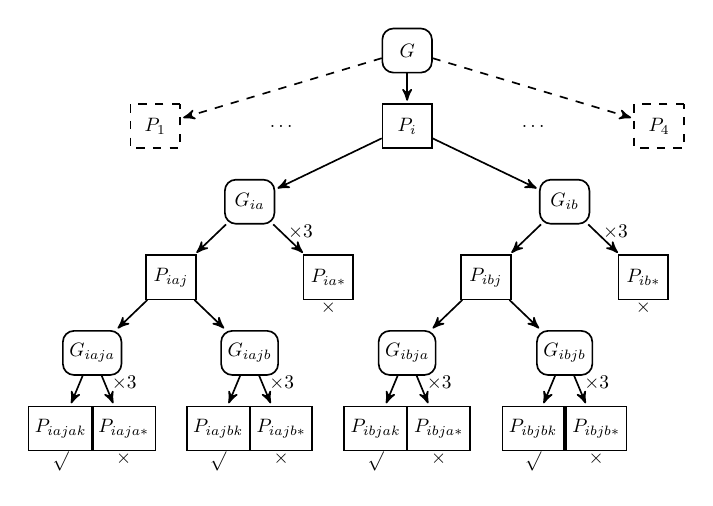
\begin{tikzpicture}[scale=0.8,level distance=1.2cm]
\tikzstyle{txt}=[scale=0.7]
\tikzstyle{planbox}=[scale=.7,draw,minimum height=0.8cm,minimum width=0.9cm]
\tikzstyle{goalbox}=[scale=.7,draw,rounded corners,minimum height=0.8cm,minimum width=0.9cm]
\tikzstyle{level 1}=[sibling distance=4.0cm] 
\tikzstyle{level 2}=[sibling distance=5.0cm] 
\tikzstyle{level 3}=[sibling distance=2.5cm]
\tikzstyle{level 4}=[sibling distance=2.5cm]
\tikzstyle{level 5}=[sibling distance=1cm]

\node[goalbox,yshift=1cm,solid] (T) {$G$}
	child[dashed] {node[planbox] (P1) {$P_1$}}
	child[solid] {node[planbox] (Pi) {$P_i$}
		child {node[goalbox] {$G_{ia}$}
			child {node[planbox] {$P_{iaj}$}
				child {node[goalbox] {$G_{iaja}$}
					child {node[planbox] {$P_{iajak}$} node[txt,below=0.3cm] {$\surd$}}
					child {node[planbox] {$P_{iaja*}$} node[txt,below=0.3cm] {$\times$}
						edge from parent node[txt,right,near start] {$\times 3$}
					}
				}
				child {node[goalbox] {$G_{iajb}$}
					child {node[planbox] {$P_{iajbk}$} node[txt,below=0.3cm] {$\surd$}}
					child {node[planbox] {$P_{iajb*}$} node[txt,below=0.3cm] {$\times$}
						edge from parent node[txt,right,near start] {$\times 3$}
					}
				}
			}
			child {node[planbox] {$P_{ia*}$} node[txt,below=0.3cm] {$\times$}
				edge from parent node[txt,right,near start] {$\times 3$}
			}
		}
		child {node[goalbox] {$G_{ib}$}
			child {node[planbox] {$P_{ibj}$}
				child {node[goalbox] {$G_{ibja}$}
					child {node[planbox] {$P_{ibjak}$} node[txt,below=0.3cm] {$\surd$}}
					child {node[planbox] {$P_{ibja*}$} node[txt,below=0.3cm] {$\times$}
						edge from parent node[txt,right,near start] {$\times 3$}
					}
				}
				child {node[goalbox] {$G_{ibjb}$}
					child {node[planbox] {$P_{ibjbk}$} node[txt,below=0.3cm] {$\surd$}}
					child {node[planbox] {$P_{ibjb*}$} node[txt,below=0.3cm] {$\times$}
						edge from parent node[txt,right,near start] {$\times 3$}
					}
				}
			}
			child {node[planbox] {$P_{ib*}$} node[txt,below=0.3cm] {$\times$}
				edge from parent node[txt,right,near start] {$\times 3$}
			}
		}
	}
	child[dashed] {node[planbox] (P4) {$P_4$}}
;
\node[txt] at ($ (P1)!.5!(Pi) $) {$\ldots$};
\node[txt] at ($ (Pi)!.5!(P4) $) {$\ldots$};

\end{tikzpicture}

\end{center}
\caption{Goal-Plan hierarchy $\T_3$. There are $2^4$ worlds whose solutions are
distributed evenly in each of the $4$ top level plans. Successful execution trace
is of length $4$. Within each sub-tree $P_i$ \BUL\ is expected to perform better
for a given world, but it suffers in the number of worlds. Overall, \CL and \BUL\
perform equally well in this structure.}
\label{fig:T3}
\end{figure}



Consider the example in Figure \ref{fig:T3}.
% %
Suppose that in some execution, plan $P_i$, for some $i \in \{1,\ldots,4\}$ is
selected in order to resolve top-goal $G$ in some world state $w_1$. The plan
involves, in turn, the successful resolution of sequential goals $G_A$ and $G_B$.
Suppose further that subgoal $G_A$ has been resolved successfully, yielding new
state $w_2$, and that plan $P_B$ has been chosen next to try and achieve the
second subgoal $G_B$.
% %
Suppose next that the first subgoal of plan $P_B$, namely $G_{B1}$ has been
successfully resolved, yielding new state $w_3$, but that the non-working plan
$P_{B2}'$ for subgoal $G_{B2}$ is selected in $w_3$ and execution thus
\emph{fails}.
% %
As there is no failure recovery, this failure will be propagated upwards in the
hierarchy, causing goals $G_{B2}$ as well as $G_B$ and top-level goal $G$ itself
fail.
% %
First of all, the failure (in world state $w_3$) must be recorded in the decision
tree of the plan where the failure originated, namely, plan $P_{B2}'$. Such plan
is in fact ``low-level,'' in that it has no subgoals and thus interacts with the
external world directly. Hence, all we can expect is to learn such interaction
over time.
% %
On the other hand, it is not so clear  whether the failure should also be
recorded in the decision trees for plans higher up in the hierarchy (e.g., plans
$P_B$ and $P_i$).






In order to discuss further \emph{which} data should be recorded \emph{where}, we
define the notion of an \textit{active execution trace}, as a sequence of the
form $G_0[P_0:w_0] \cdot G_1[P_1:w_1] \cdot \ldots \cdot G_n[P_n:w_n]$, which
represents the sequence of currently active goals, along with the plans which
have been selected to achieve each of them, and the world state in which the
selection was made---plan $P_i$ has been selected in world state $w_i$ in order
to achieve the $i$-th active subgoal $G_i$.
% %
In our example, the trace at the moment of failure is as follows: \[
\lambda=G[P_i:w_1] \cdot G_B[P_B:w_2] \cdot G_{B2}[P_{B2}':w_3]. \]


So, when the final goal of $\lambda$ fails, namely $G_{B2}$, it is clear that the
decision tree of the plan being used to achieve such goal ought to be updated,
and a failure should be recorded for the world state $w_3$ against 
the decision tree attached to plan $P_{B2}'$.  
%%
By recording every outcome for the lowest plans, i.e., plans with no subgoals,
the system eventually learns how such plans performs in the environment.
%%
% Although it may be the case
% that the plan usually succeeds in the situation in which it was chosen, and failure is
% simply due to some non-determinism (or in the general case, actions of other
% agents, interactions, etc.), there is no way to determine this and the learning
% process will eventually recognise such cases as ``noise.''
% %

What is more difficult to determine is whether the decision trees of plans
associated with \emph{earlier goals} in $\lambda$ should also be updated.
% %
More concretely, should failure cases in world states $w_2$ and $w_1$ be recorded
against plans $P_B$ and $P_i$, respectively?
% %
The point is that it is conceivable that the failure of subgoal $G_{B2}$ in plan
$P_B$, for instance, could indeed have been avoided, had the alternative plan
$P_{B2}$, been chosen instead. Therefore, recording a failure against plan $P_B$
would not not be justified---it is not true that plan $P_{B}$ is a ``bad'' one
when in world state $w_3$.
% %
Informally, one could argue that it is more appropiate to \emph{wait} before
recording failures against a plan until one is reasonably confident that
subsequent choices down the goal-plan tree hierarchy were ``well informed.'' In
our case, if the agent knows that the plan selection for goal $G_{B2}$ was as
good and informed as possible, then recording the failure for world $w_2$ in plan
$P_B$ would also be justified. Similarly, if the agent considers that the plan
selection for subgoal $G_B$ was an informed choice, then recording the failure
for world $w_1$ against $P_i$'s decision tree would be justified too.


\newcommand{\procedurefont}[1]{\mathsf{#1}}
\newcommand{\StableGoal}{\procedurefont{StableGoal}}
\newcommand{\RecordTrace}{\procedurefont{RecordFailedTrace}}
\newcommand{\RecordWorldDT}{\procedurefont{RecordWorldDT}}




The judgment as to whether plan choices were sufficiently ``well informed,'' is
however not a trivial one.  A plan $P$ is considered to be \emph{stable} for a
particular world state $w$ if the rate of success of $P$ in $w$ is changing below
a certain threshold $\epsilon$. In such a case, the agent can start to build
confidence about the applicability level of $P$. The stability notion extends to
goals as follows: a goal is considered \emph{stable} for world state $w$ if all
its relevant plans are stable for $w$.
% %
When a goal is stable, we regard the plan selection for such goal as a ``well
informed'' one. Thus, a plan failure is recorded in the plan if the subgoal that
failed is stable for the world it was meant to be resolved in. In our example, we
record the failure in plan $P_B$ ($P_i$) if goal $G_B$ ($G_B$) is deemed stable
in world state $w_3$ ($w_2$), that is, if the selection of option $P_{B2}'$
($P_B$) was an informed one.



The $\RecordTrace$ algorithm below shows how a failed execution run $\lambda$ is
recorded. Function
$\StableGoal(G,w,k,\epsilon)$ returns true iff goal $G$ is considered \textit{stable} for world state $w$, under change of
success rate thresholds $0 < \epsilon \leq 1$ and minimal number of executions $k
\geq 0$.
 
 \renewcommand{\algorithmiccomment}[1]{\hfill \texttt{\small // #1}}
 \newcommand{\assign}{\mbox{:=\ }}
 \begin{algorithm}[h]
	\caption{$\RecordTrace(\lambda,k,\epsilon)$}\label{algo:record_failed_exec}
	\label{alg:NDS}
  \begin{algorithmic}[1]
    \REQUIRE $\lambda=G_0[P_0:w_0] \cdot \ldots \cdot G_n[P_n:w_n]$; $k\geq0$;
    $\epsilon > 0$ \ENSURE Propagates DT updates for plans

	\STATE $\RecordWorldDT(P_n,w_n,\failure)$

    \IF{$\StableGoal(G_n,w_n,k,\epsilon) \land |\lambda|>1$}
    	 \STATE $\lambda' \assign G_0[P_0:w_0] \cdot \ldots \cdot
    				G_{n-1}[P_{n-1}:w_{n-1}]$
    	\STATE $\RecordTrace(\lambda',k,\epsilon)$ \COMMENT{recursive call}
    \ENDIF
  \end{algorithmic}
\end{algorithm}

 
The algorithm starts by recording the failure against the last plan $P_n$ in the
trace.
% %
Next, if the choice of executing plan $P_n$ to achieve goal $G_n$ was deemed an
informed one (that is, goal $G_n$ was stable for $w_n$), then the procedure
should be repeated for the previous goal-plan nodes, if any.
% %
If, on the other hand, the last goal $G_n$ in the trace is not considered stable
enough, the procedure terminates and no more failure data is assimilated.
% %
Observe that, in order to update the decision tree of a certain plan that was
chosen along the execution, it has to be the case that the (failed) decisions
taken during execution must have all been informed ones.



So, in the remaining of the paper, we shall consider two learning approaches
compatible with the framework developed in the previous section. The first, which
we call \emph{aggressive concurrent learning} (\CL), corresponds to the more
traditional approach where all data is always assimilated by the learner, that
is, we take $\epsilon = 1$ and $k = 0$. In other words, every plan and every goal
is always considered stable and, as a result, a failure in a plan is always
recorded. The assumption is that misleading information, as discussed above, will
eventually disappear as noise.
% %
The second one, which we refer to as \emph{bottom-up learning} (\BUL), is more
cautious and records a failure execution experience when some stability on
decisions is deemed, that is, $\epsilon > 0$. In our work, we have taken
$\epsilon = 0.3$ and $k = 3$, that is, the context condition of a plan is
considered stable (for a world state) if at least $3$ past execution experiences
have been recorded and the rate of success has lately been changing less than
$0.3$.
% %
Note that the lower $\epsilon$ is and the higher $k$ is, the more conservative
the agent is in considering its decisions ``well informed.''

In the following section, we shall explore these two approaches against
different programs with different structures.






%%%%%%%%%%%%%%%%%%%%%%%%%%%%%%%%%%%%%%%%%%%%%%%%%%%%
\section{Experimental Results}\label{sec:experiments}
%%%%%%%%%%%%%%%%%%%%%%%%%%%%%%%%%%%%%%%%%%%%%%%%%%%%

%\begin{figure*}[t]
%\begin{center}
%\subfigure[Structures $\T_1$ (crosses) and $\T_3$ (circles)]{\label{fig:tree01_result}
%\begin{tikzpicture}[x=0.0075cm,y=4cm]
%	% DRAW AXES LINES
%    \draw[->,xshift=0] (0,0) -- coordinate (x axis mid) (1050,0);
%    \draw[->,xshift=0] (0,0) -- coordinate (y axis mid) (0,1.1);

%	% DRAW AXES NUMBERS
%    \foreach \x/\xtext in {0/0,1.5/200,3/400,4.5/600,6/800,7.5/1000}
%        \draw [xshift=0cm](\x cm,1pt) -- (\x cm,-3pt)
%            node[anchor=north] {$\xtext$};
%    \foreach \y/\ytext in {0/,1/25,2/50,3/75,4/100}
%        \draw (-1pt,\y cm) -- (0pt,\y cm) node[anchor=west] {$\ytext$};

%	% WRITE AXES LABELS
%    \node[above,xshift=3cm] at (x axis mid) {\# Iterations};
%%     \node[below=.5cm] at (x axis mid) {Iterations};
%    \node[above,shift={(0.8cm,2cm)}] at (y axis mid) {\% Success};

%	% PLOT bul DATA TEST 01
%    \draw[-] plot[mark=x,mark size=3,smooth,mark options={color=black}] 
%			file {data/previous/failtest01-bul.data};
%	% PLOT cl DATA TEST 01
%    \draw[dashed,-] plot[mark=x,mark size=3,smooth,mark options={color=black}] 
%			file {data/previous/failtest01-cl.data};

%	% PLOT bul DATA TEST 18
%    \draw[-] plot[mark=*,mark size=1,smooth,mark options={color=black}] 
%			file {data/previous/failtest18-bul.data};
%	% PLOT cl DATA TEST 18
%    \draw[dashed,-] plot[mark=*,mark size=1,smooth,mark options={color=black}] 
%			file {data/previous/failtest18-cl.data};
%\end{tikzpicture}
%}
%\qquad
%\subfigure[Structure $\T_2$]{\label{fig:tree08_result}
%\begin{tikzpicture}[x=0.00121cm,y=4cm]
%	% DRAW AXES LINES
%    \draw[->,xshift=0] (0,0) -- coordinate (x axis mid) (6300,0);
%    \draw[->,xshift=0] (0,0) -- coordinate (y axis mid) (0,1.1);

%	% DRAW AXES NUMBERS
%    \foreach \x/\xtext in {0/0,1.452/1200,2.904/2400,4.356/3600,5.808/4800,7.26/6000}
%        \draw [xshift=0cm](\x cm,1pt) -- (\x cm,-3pt)
%            node[anchor=north] {$\xtext$};
%    \foreach \y/\ytext in {0/,1/25,2/50,3/75,4/100}
%        \draw (-1pt,\y cm) -- (0pt,\y cm) node[anchor=west] {$\ytext$};

%	% WRITE AXES LABELS
%    \node[above,xshift=3cm] at (x axis mid) {\# Iterations};
%%     \node[below=.5cm] at (x axis mid) {Iterations};
%    \node[above,shift={(0.8cm,2cm)}] at (y axis mid) {\% Success};
%%     \node[left=0.5cm,rotate=90,xshift=1cm] at (y axis mid) {Success Income};

%	% PLOT STABLE DATA
%    \draw[-] plot[mark=*,mark size=0,smooth,mark options={color=black}] 
%			file {data/previous/failtest08-bul.data};
%	% PLOT STABLE DATA
%    \draw[dashed,-] plot[mark=x,mark size=0,smooth,mark options={color=black}] 
%			file {data/previous/failtest08-cl.data};
%\end{tikzpicture}
%}
%\caption{Agent performance under \BUL\ and \CL\ schemes. Solid lines
%represent agent performance under the \BUL\ approach; dashed lines represent agent performance under
%the \CL\ approach. Each point stands for the average of the last $20$ executions.}
%\end{center}
%\end{figure*}

	

In order to explore the difference between \BUL\ and \CL, we set up testbed
programs composed of several goals and plans combined in a hierarchical manner
and yielding goal-plan tree structures of different shapes.\footnote{We have
implemented the learning agent system in the \JACK\ BDI platform
\cite{Busetta99jack}. The fact that \JACK\ is a Java-based system and
provides powerful meta-level reasoning capabilities, allows us to integrate \weka\ and
probabilistic plan-selection mechanisms with not much effort. Nonetheless, all
the results are independent on this and any other BDI agent system could
have been used.}
% %
In particular, we crafted goal-plan tree structures representing different
meaningful cases of BDI programs with one main top-level goal, i.e., the event to
be resolved. In addition, each structure enjoys the, generally desirable,
\emph{coverage} property, under which for every possible situation, (i.e., world
state), there is always a way of addressing the main goal, i.e., there is at
least one successful execution of the top-level event, provided the right plan
choices are made. Observe that such successful (plan) choices may be different
for different world states.
% , as know-how information is generally predicated on the situation it is
% applied in. %
When it comes to describing the possible (observable) world states, we have used
a set of logical (binary) propositions, representing the so-called fluent or
features of the environment that are observable to the agent (e.g., fluent
proposition $\mathit{DoorLocked}$ states whether the door is believed open or
not).
% %
Finally, we assume the agent is acting in a non-deterministic environment, in
which actions that are expected to succeed, may still fail with some (small)
probability. In most of our experiments, we assumed a $.1$ probability of
uncontrolled failure for such actions.\footnote{See Discussion section on how our
results generalize to a framework with world state built from non-binary fluents
and with more complex accounts for stochastic actions.}
% %




The experiments consisted in posting the top-level goal repetitively under random
world states, running the corresponding  BDI learning agent, and finally
recording whether the execution terminated successfully or not.
% %
We calculated the average rate of success of the goal every some fixed
number of iterations (in our case $20$), and investigated how such rate evolved
as the agent refined the context condition of plans.
% %%
We ran the tests under both a \BUL-based agent and a \CL-based agent,
ensuring the same sampling of random world states for each agent.

\begin{figure}[t]
\begin{center}
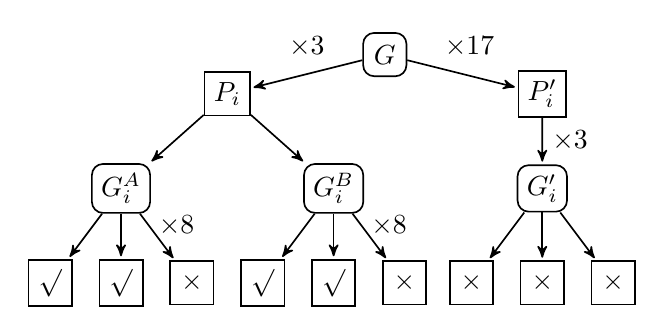
\begin{tikzpicture}[level distance=1.2cm]

\tikzstyle{planbox}=[draw,minimum height=0.55cm,minimum width=0.55cm]
\tikzstyle{goalbox}=[draw,rounded corners,minimum height=0.55cm,minimum width=0.55cm]

\tikzstyle{level 1}=[sibling distance=4cm,level distance=0.5cm] 
\tikzstyle{level 2}=[sibling distance=2.7cm,level distance=1.2cm]
\tikzstyle{level 3}=[sibling distance=.9cm]
\tikzstyle{level 4}=[sibling distance=1cm]

\node[goalbox] (T) {$G$}
   child[solid] {node[planbox] (1) {$P_i$}
      	child {node[goalbox] (11) {$G_i^A$}
			child {node[planbox] {$\surd$}
			}
			child {node[planbox] {$\surd$}
			}
			child {node[planbox] {$\times$}
				edge from parent node[right,near start] {$\times 8$}
			}
	  	}
      	child {node[goalbox] (11) {$G_i^B$}
			child {node[planbox] {$\surd$}
			}
			child {node[planbox] {$\surd$}
			}
			child {node[planbox] {$\times$}
				edge from parent node[right,near start] {$\times 8$}
			}
	  	}
	edge from parent node[above left, near start] {$\times 3$}
   }
   child[solid] {node[planbox] (2) {$P_i'$}
      child {node[goalbox] (22) {$G_i'$} 
	child {node[planbox] {$\times$}}
	child {node[planbox] {$\times$}}
	child {node[planbox] {$\times$}}
	edge from parent node[right] {$\times 3$}
	}
   edge from parent node[above right,near start] {$\times 17$}};

% \draw (T) -- (1) node (aux1) [coordinate,midway]{};
% \draw (T) -- (2) node (aux2) [coordinate,midway]{};
% \draw (aux1) .. controls +(0.3,-0.3) and +(-0.3,-0.3).. (aux2)
% 			node[midway,above] {OR};

% \draw (1) -- (11) node (aux21) [coordinate,midway]{};
% \draw (1) -- (12) node (aux23) [coordinate,midway]{};
% \draw (aux21) .. controls +(0.25,-0.25) and +(-0.25,-0.25).. (aux23)
% 			node[midway,above] {AND};

% \node[below left of=T,text width=2cm,xshift=-3cm] (label)
% 		{$P_i$: plan \\ $G_i$: goals \\ $SG_i$: sub-goals};
\end{tikzpicture}

\end{center}
\caption{Goal-plan tree hierarchical structure $\T_1$. To succeed, an agent is thus required to make
two correct choices, including selecting $P$ at the top-level.}
\label{fig:T1}
\end{figure}


From our set of experiments, we have selected three hierarchical structures that
best illustrate the results that we have obtained, namely:
% %
\begin{description}
\item[(Tree $\T_1$; Figure~\ref{fig:T1})] For each world state, the goal has
few plans that can succeed (plans $P_i$), but many other options of comparable
complexity that are bound to fail (plans $P_i'$). 
%%
Under this type of structure, an \CL-based agent will generally perform better 
than an agent using the learning \BUL\ approach.

\item[(Tree $\T_2$; Figure~\ref{fig:T2})] For each world state, the goal has
one plan that can succeed (plan $P$), and a few others that would fail.
However, the plan containing the solution is of substantial higher-complexity. 
%%
In this structure, a \BUL-based agent will outperform an \CL-based one.
% A structure in which \BUL\ is
% expected to have important advantages over \CL, since the latter may wrongly consider a
% top-level plan as a failing plan whereas there is a solution encoded
% under it. 

\item[(Tree $\T_3$; Figure~\ref{fig:T3})] This stands for a ``balanced''
structure that ends up providing different advantages for both \BUL\ and \CL\ in
different parts of the tree.
\end{description}


% In summary, we found that whereas the agent performance under the \BUL\ and \CL\
% approaches is comparable on the first and third cases, the \BUL\ scheme provides
% substantial benefits in the second case. What is more important, if we consider
% agents that may choose not to consider a plan at all when its chances of success
% are believed very low, then the \CL\ approach collapses completely whereas the
% \BUL\ is robust enough to maintain performance.

% For lack of space, we shall only give the form of tree $\T_1$ and informally
% explain the characteristics of the other two.

Let us next discuss each of the plan-goal structures and how the performance of
\BUL-based and \CL-based agents compare.


Under a structure like $\T_1$, the agent basically has several options of the
comparable complexity to resolve the top-level goal $G$ in certain world state,
in our case, $20$ options. However, most of such options---$17$ in our example;
plans $P_i'$---would inevitably lead to failure.
% %
The benefit of using the \CL\ approach comes from the fact that the agent will
decrease the probability of selecting each of those $17$ failing plans as soon as
they fail for the first time. In contrast, \BUL\ would require several failed
experiences of each of those ``bad'' top-level options before decreasing their
probability of selection---to update the decision tree of plan $P_i'$, \BUL\
requires each of their three subgoals to be ``stable.''
% %%
As we expected the \CL\ scheme did perform better in our experiments, in that it
achieved better success rate earlier; see Figure~\ref{fig:T1_result}.
% %
Note then that whereas the agent under the \CL\ approach reaches $50\%$ success
after $1000$ iterations, it takes more than double for \BUL\ to achieve that
performance.
% %
Eventually, both approaches will yield optimal performance. Observe that optimal
performance amounts to a success rate of $81\%$, as the environment fails with
probability $.1$ for every (working) action and each successful plan involves
two actions.


\begin{figure}[t]
\begin{center}
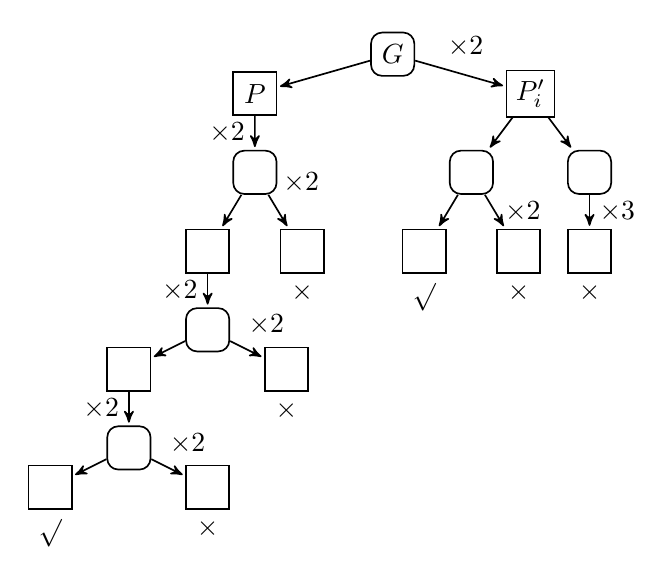
\begin{tikzpicture}[level distance=1.2cm]
\tikzstyle{txt}=[scale=.9]

\tikzstyle{succ}=[label=below:$\surd$]
\tikzstyle{fail}=[label=below:$\times$]


\tikzstyle{planbox}=[draw,minimum height=0.55cm,minimum width=0.55cm]
\tikzstyle{goalbox}=[draw,rounded corners,minimum height=0.55cm,minimum width=0.55cm]

\tikzstyle{level 1}=[sibling distance=3.5cm,level distance=0.5cm] 
\tikzstyle{level 2}=[sibling distance=1.5cm,level distance=1.0cm]
\tikzstyle{level 3}=[sibling distance=1.2cm,level distance=1.0cm]
\tikzstyle{level 4}=[sibling distance=1.2cm,level distance=1.0cm]
\tikzstyle{level 5}=[sibling distance=2.0cm,level distance=0.5cm]
\tikzstyle{level 6}=[sibling distance=1.2cm,level distance=1.0cm]
\tikzstyle{level 7}=[sibling distance=2.0cm,level distance=0.5cm]
\tikzstyle{level 8}=[sibling distance=1.2cm,level distance=1.0cm]

\node[goalbox] (T) {$G$}
   child[solid] {node[planbox] (1) {$P$}
      child {node[goalbox] (11) {\phantom{$G$}}
		child {node[planbox] {\phantom{$P$}}
			child {node[goalbox] {\phantom{$G$}}
				child {node[planbox] {\phantom{$P$}}
					child {node[goalbox] {\phantom{$G$}}
						child {node[planbox,succ] {\phantom{$P$}}}
						child {node[planbox,fail] {\phantom{$P$}}
							edge from parent node[above right,near start] {$\times 2$}
						}
						edge from parent node[left] {$\times 2$}
					}
				}
				child {node[planbox,fail] {$\phantom{P}$}
					edge from parent node[above right,near start] {$\times 2$}
				}
		               edge from parent node[left] {$\times 2$}
			}
		}
		child {node[planbox,fail] {\phantom{$P$}}
			edge from parent node[above right,near start] {$\times 2$}
		}
               edge from parent node[left] {$\times 2$}
	}
   }
   child[solid] {node[planbox] (2) {$P_i'$}
      	child {node[goalbox] (11) {\phantom{$G$}}
			child {node[planbox,succ] {$\phantom{P}$}}
			child {node[planbox,fail] {$\phantom{P}$} 
		               edge from parent node[right] {$\times 2$}
			}
	}
      	child {node[goalbox] {\phantom{$G$}}
			child {node[planbox,fail] {$\phantom{P}$} 
		               edge from parent node[right] {$\times 3$}
			}
	}
	edge from parent node[above right, near start] {$\times 2$}
};
\end{tikzpicture}



\end{center}
\caption{Goal-plan tree hierarchical structure $\T_2$.}
\label{fig:T2}
\end{figure}


\begin{figure*}[t]
\begin{center}
\subfigure[Structure $\T_1$]{\label{fig:T1_result}
%!TEX root = ../dsingh-aamas10-poster.tex
\begin{tikzpicture}[x= 0.008cm,y=9cm]
	\definecolor{darkblue}{rgb}{0.1,0.1,0.5}
	\definecolor{darkred}{rgb}{0.8,0.0,0.1}
    % Draw the axes and grid lines
    \draw[-] (0,0) -- (0,1) -- (2000,1) -- (2000,0) -- cycle; 
    \draw[-,thin, dotted, ystep=0.2, xstep=2000] (0,0) grid (2000,1);
    \foreach \x in {500, 1000, 1500}  \draw [-,xshift=0](\x,4pt) -- (\x,-1pt);
    \foreach \y in {0.0,0.2,0.4,0.6,0.8,1.0}  \draw [-,yshift=0](4pt,\y) -- (-1pt,\y);
    \foreach \x/\xtext in {500/500, 1000/1000, 1500/1500} \node at (\x,0) [below] {\xtext};
    \foreach \y/\ytext in {0.0,0.2,0.4,0.6,0.8,1.0}  \node at (0,\y) [left] {\ytext};
    \node at (0,1.15) {Success};
    \node at (1650,0.1) {Iterations};
    \draw[-,darkred] plot[mark=x,mark size=10,mark options={color=darkred}] 
			file {figs/data/test01v3gm.CP.tikzdata};
    \draw[-,darkblue] plot[mark=o,mark size=6,mark options={color=darkblue}] 
			file {figs/data/test01v3gm.SP.tikzdata};
    % Also draw the expected convergence: 0.9^4 actions=0.6561
    \draw[dashed,-,yshift=0](0,0.81) -- (2000,0.81);
	\node at (2300,0.5) {$\mathcal{T}1$};
\end{tikzpicture}

}
\qquad
\subfigure[Structure $\T_2$]{\label{fig:T2_result}
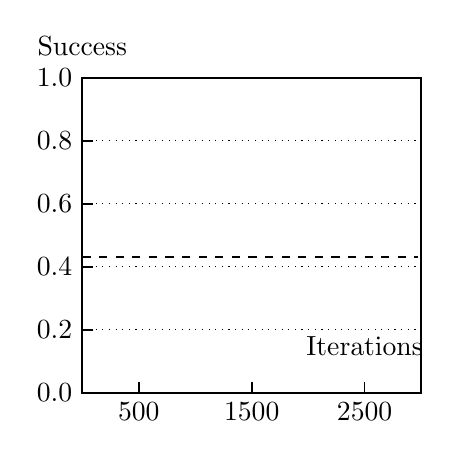
\begin{tikzpicture}[x=0.00143cm,y=4cm]
    % Draw the axes and grid lines
    \draw[-] (0,0) -- (0,1) -- (3000,1) -- (3000,0) -- cycle; 
    \draw[-,thin, dotted, ystep=0.2, xstep=3000] (0,0) grid (3000,1);
    \foreach \x in {500, 1500, 2500}  \draw [-,xshift=0](\x,4pt) -- (\x,-1pt);
    \foreach \y in {0.0,0.2,0.4,0.6,0.8,1.0}  \draw [-,yshift=0](4pt,\y) -- (-1pt,\y);
    \foreach \x/\xtext in {500/500, 1500/1500, 2500/2500} \node at (\x,0) [below] {$\xtext$};
    \foreach \y/\ytext in {0.0,0.2,0.4,0.6,0.8,1.0}  \node at (0,\y) [left] {$\ytext$};
    \node at (0,1.1) {Success};
    \node at (2500,0.15) {Iterations};
    \draw[-] plot[mark=triangle,gray,mark size=3,mark options={color=gray}] 
			file {data/test05v3gm.CP.tikzdata};
    \draw[-] plot[mark=o,gray,mark size=2,mark options={color=gray}] 
			file {data/test05v3gm.SP.tikzdata};
    % Also draw the expected convergence: 0.9^8 actions=0.43046
    \draw[dashed,-,yshift=0](0,0.43046) -- (3000,0.43046);

\end{tikzpicture}

}
\qquad
\subfigure[Structure $\T_3$]{\label{fig:T3_result}
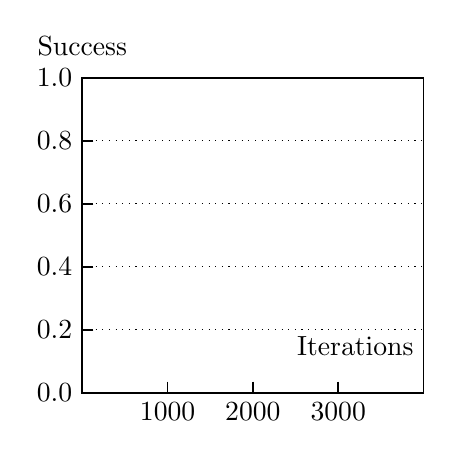
\begin{tikzpicture}[x=0.00108cm,y=4cm]
    % Draw the axes and grid lines
    \draw[-] (0,0) -- (0,1) -- (4000,1) -- (4000,0) -- cycle; 
    \draw[-,thin, dotted, ystep=0.2, xstep=4000] (0,0) grid (4000,1);
    \foreach \x in {0,1000,...,4000}  \draw [-,xshift=0](\x,4pt) -- (\x,-1pt);
    \foreach \y in {0.0,0.2,0.4,0.6,0.8,1.0}  \draw [-,yshift=0](4pt,\y) -- (-1pt,\y);
    \foreach \x/\xtext in {1000/1000, 2000/2000, 3000/3000} \node at (\x,0) [below] {$\xtext$};
    \foreach \y/\ytext in {0.0,0.2,0.4,0.6,0.8,1.0}  \node at (0,\y) [left] {$\ytext$};
    \node at (0,1.1) {Success};
    \node at (3200,0.15) {Iterations};
    \draw[-] plot[mark=triangle,gray,mark size=3,mark options={color=gray}] 
			file {data/testImpactvars.CP.tikzdata};
    \draw[-] plot[mark=o,gray,mark size=2,mark options={color=gray}] 
			file {data/testImpactvars.SP.tikzdata};

\end{tikzpicture}

}
\caption{Agent performance under \BUL\ (circles) and \CL\ (triangles) schemes.
Each point represents results from $5$ experiment runs using a moving average of $100$ samples.}
\end{center}
\end{figure*}


The second structure $\T_2$ that we considered amounts to simplifying
each plan $P_i'$ to be just a single action that always fails and
making the goal-tree hierarchy below plan $P$ more complex, that is,
deeper and with more goals.\footnote{For lack of space, we do not show
this structure.}
% \footnote{For lack of space, we do not show
% this structure, but will be included in the final version.}
%
Under such hierarchy, the agent needs to make four correct plan
choices to result in a successful execution; there are also many
chances for the agent to fail under $P$.
%
Although one would expect \BUL\ to yield better agent performance than
\CL, the difference is enormous. Figure \ref{fig:T2_result} shows
that while the \BUL\ approach, achieves optimal performance in around
$100$ iterations, the \CL\ scheme, requires around $5000$ execution
experiences.  
%
The reason is clear: since there are more chances to fail plan $P$
initially, \CL\ marks this plan ``bad,'' causing plans $P_i'$ (which
are all non-working) to be selected at least once in preference to
trying $P$ again. On the other hand, \BUL\ would not consider $P$
``bad'' even when failing it, since it is aware that decisions made 
below were not informed enough. Consequently $P$ will continue to be
explored with equal likelihood to the $P_i'$.
% *** Sentence below could be cut - its an aside...
%
As a matter of fact,
provided adequate parameters are used for checking stability, \BUL\
would only record failed execution traces in plan $P$ if the
environment happened to fail unexpectedly: if the decisions were
informed and the environment cooperated, then the execution is
expected to succeed. 
%
Notice that optimal behavior amounts to less than a $75\%$ rate of
success, since the agent needs to ultimately perform four actions,
each of them having a probability of success of $90\%$ when performed
in the real world. 

Let us now consider the third hierarchical structure $\T_3$, depicted
in Figure \ref{fig:T3}. In this case, the top-level goal $G$ has
five relevant plans, which are all ``complex,'' that is, they all have
several levels and multiple goals and plans. However, only one
particular path in this hierarchy will lead to a successful 
execution for a particular world state. 
Among other things, this means that at the top-level the agent ought
to select the right plan, all the other four plans are bound to fail
eventually. 
%
We argue that this is the typical case in most BDI agent systems, in
that for each goal, the agent may have several strategies, but each
one is crafted to cover uniquely a particular subset of states.
%
From the two learning approaches we are considering, structure $\T_3$
provides advantages for both of them, in different parts of the
tree. The \CL\ scheme is expected to learn faster the inadequacy 
of the four non-working top-level programs, but the \BUL\ would better
explore, and find a solution, within the working top-level plan.
%
This balance is corroborated by the fact that both agents have
comparable performance, with \BUL\ yielding improved behavior slightly
quicker (see Figure \ref{fig:T1_result}, circle marked). 

However, we are currently considering all plans as potentially
applicable and worth trying - even when there is a very low chance of
success. Given that executing a plan is often not cost-free in real
systems, it is likely that the plan selection mechanism would in fact
not execute plans with too low a probability of success. This would
presumably hurt \CL.
% 
In order to demonstrate this we modified the probabilistic plan
selection explained in Section \ref{sec:framework} so that the \JACK\
agent does not consider plans whose chance of success are below 0.2.
In this experiment we also removed the non-determinism---actions
always fail or succeed in each world state.\footnote{Managing the
non-determinism without continuing to, with some probability, try all
plans, requires a more sophisticated mechanism than a simple
probability check, to avoid randomly cutting off options that happen
to have failed on one iteration. However in the interests of
simplicity we deal with the simplified case.}
%
The differences, shown in Figure \ref{fig:T2_result} are striking.

Using the structure 
$\T_3$ we  found that whereas \BUL\ maintains its performance (and in
fact slightly improves, as failing leaf plans are discarded earlier
than before thus reaching optimal performance around $100$
iterations), the \CL\ approach is never able to learn and eventually
is guaranteed to always fail the top-level goal.

The explanation for this wrong behavior under \CL\ is as
follows. Initially, the agent tries all top-level plans for the
top-level goal. Because of their complexity, it is extremely unlikely
that the set of correct choices are made randomly. Thus their
executions fail.
This causes \CL\ to decrease the feasibility of all plans
tried, including the top-level ones. As this will likely happen
for several iterations, eventually all plans for a goal reach a probability of
success lower than required, thus
running out of options, failing the goal in question, and propagating
the failure up in the hierarchy. Eventually, the top-level plans end
up with low expectations of success and are ruled out.
This will give no options to try and the goal will always
fail.\footnote{Such behavior does not arise in the original
system because even if all plans have extremely low success chances,
the agent would pick one anyway. As a result, the successful path
would be eventually be found and plans' context conditions would start
``recovering.''}

We conclude then that overall \BUL\ clearly exhibits more robust
behaviour. In addition, in some structures \CL\ can pay significant
costs, by considering some strategies as not viable too early. In
those structures where \BUL\ performs worse, the difference is
relatively small. 






%%%%%%%%%%%%%%%%%%%%%%%%%%%%%%%%%%%%%%%%%%%%%%%%%%%%
\section{Informed Plan Selection}\label{sec:coverage}
%%%%%%%%%%%%%%%%%%%%%%%%%%%%%%%%%%%%%%%%%%%%%%%%%%%%

\Omit{
The first part of this paper addresses the task of determining when
decisions along the active execution trace may be considered
\textit{informed enough} for outcomes to be included as learnable
instances for each \dt in that trace. For this we contrast two
schemes, \CL\ and \BUL\ - and show that the conservative \BUL\
approach delivers more robust performance than the simpler \CL\
approach for the cases considered. For both approaches, the same
probabilistic function $E$ (or exploration strategy) was used to make
the plan selection at each junction of the active execution trace.  

In subsequent work we keep the \CL\ and \BUL\ recording methods constant, and adjust the probabilistic plan selection function $E$ to evaluate the impact on the learning outcome. Motivated by the polarity between the two approaches, we consider if an informed probabilistic selection function $E'$ may be constructed to yield a \textit{middle ground} approach that applies better in the general case. This would be valuable since if a \CL+$E'$-based approach yields comparable performance to any \BUL+$E^*$-based approach, then the former is preferred as \CL\ is much simpler than \BUL. Interestingly we find that such a formulation is possible and that an informed exploration strategy that leverages both the domain knowledge (inherent in the goal-plan tree hierarchy) as well as the ongoing learning (agent's experience so far) can combine the benefits of both \CL\ and \BUL.
}

In the new approach instead of using the stability measure to ensure that we only
record results that we are confident in, we instead modify our plan selection
procedure to take account of how confident we are in the current decision tree.
If the decision tree probability is based on very sparse exploration of the
relevant subspace then we should be less confident in this information than if
the space is thoroughly explored. We note that the stability measure ensures that
failure information is not recorded in the decision tree until the tree is
adequately explored. Our new approach instead influences how we use the decision
trees for plan selection.

We start by quantifying the quality of (or our \textit{confidence} in)
the hypotheses of a \dt for a unknown subspace $S$ of world states
$[w_1 \ldots w_n] \in W$ \footnote{Note that in general not every plan
  can be selected in every world state. Subspace $S$ refers to the
  subset of world states where the plan may be selected.}. At the
beginning of a run we have no learnable instances and for a given
goal-plan tree node $T$ our probability of success $p_T(w)$ in world
$w \in S$ is given by the default probability $0.5$. After the first
instance is recorded, the \dt will generalise the result to the full
space of $S$ (i.e. $\forall w \in S$) leading to likely
\textit{mis-classification}. Intuitively we know that as more and more
$w \in S$ are witnessed and recorded, the \dt's classification over
$S$ will improve. 

\Omit{Our two approaches may be described in terms of
confidence as follows: \CL\ always assumes full confidence in the \dt
but suffers from misclassification errors (that are eventually
rectified through subsequent learning from misinformed choices); \BUL\
uses the static $\epsilon$ and $k$ values to determine the boundary
for our confidence in the \dt (with the trade-off that for the period
of no confidence the best we can do is use $0.5$). 
}

What we want is to compute a smooth transition
from zero-confidence in the \dt classification to full-confidence,
based on experience. We identify two orthogonal properties,
\textit{choices} and \textit{subspace} that are integral to informed
decision making by 
%the learning nodes in 
our agent. Choices refer to
the set of all statically computable execution paths \textit{below} a
goal node in the goal-plan tree hierarchy. Subspace refers to the set
of all worlds that are learnable for the \dt at that node. Defined in
those terms, we label a \dt \textit{not informed} if no choices have
been recorded in any world of the subspace, or \textit{fully informed}
when all choices have been covered in every world of the subspace. 

%In fact, we can construct a measure of our confidence in the \dt based on
%the degree of \textit{coverage} of all choices in all subspace
%associated worlds. 
%In other words, \textit{coverage} may be defined as the fraction  
% *** not sure what you wanted to say in above - it was left as a
% hanging sentence... ???

We define an equation for determining plan selection probability that
is influenced by this confidence measure based on the level of
\textit{coverage} of all choices in all subspace associated worlds:

\begin{equation}
\label{eqn:coverage}   
E': p'_T(w)= 0.5 + \left[  c_T(S) *  \left( p_T(w) - 0.5 \right)  \right]
\end{equation}

%Equation \ref{eqn:coverage} shows how a confidence measure based on
%coverage may be used to modify the final plan selection
%probability. 
The idea here is to bias the \dt classification (probability
of success) of world $w$ in node $T$ given by $p_T(w) \in [0 \ldots
1]$ with the coverage $c_T(S) \in [0 \ldots 1]$ of subspace $S$ given
$w \in S$. Initially the coverage is zero, so the revised probability
$p'_T(w) = 0.5$ the default probability of success. As coverage
$\rightarrow 1$, the revised probability $p'_T(w) \rightarrow p_T(w)$
the \dt classification. This gives a progressive transition to the \dt
classification as more experience is acquired (Figure
\ref{fig:coverage-surface}). 

\begin{figure}[ht]
   \centering
   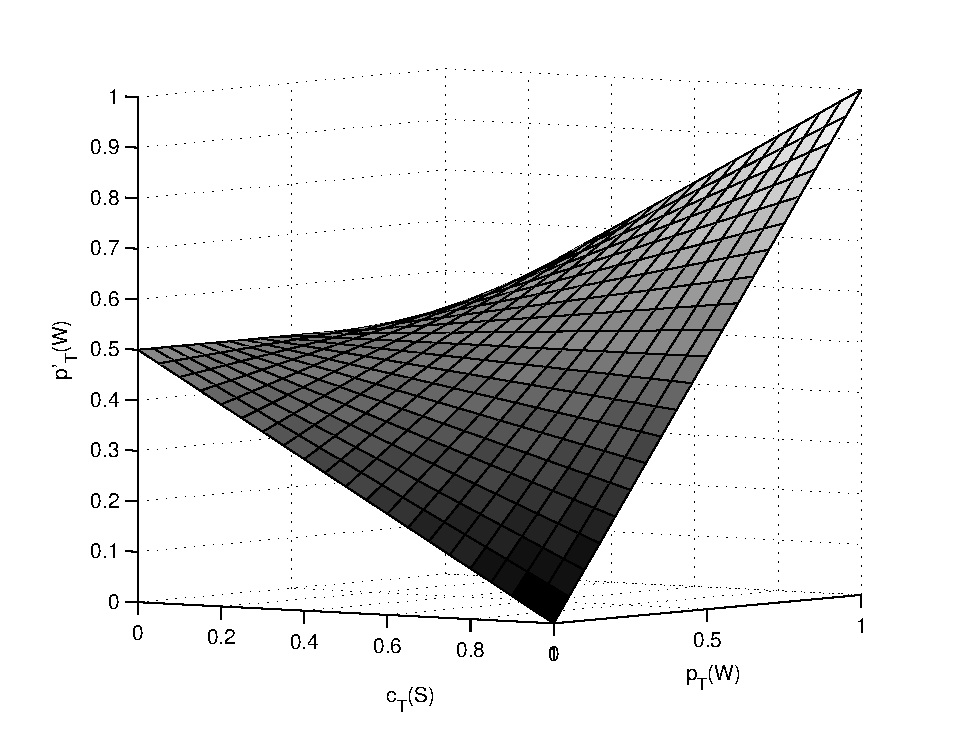
\includegraphics[width=\columnwidth]{figs/coverage-surface}
   \caption{How confidence (coverage) is used to adjust \dt classification for plan selection.}
   \label{fig:coverage-surface}
\end{figure}


The coverage $c_T(S)$ itself is calculated and stored each time a
result is recorded for node $T$. The calculation is performed in turn
for each node in the active execution trace starting at the leaf node
where the failure occurred, and the coverage is updated progressively
up the tree hierarchy. Full coverage at a node $T$ requires $C(T)*|S|$
unique samples where $C(T)$ is the total number of choices below $T$
and $|S|$ is the number of worlds in the subspace. Practically
however, it takes significantly less since choices below $T$ are
effectively AND/OR trees, and each time an AND node fails the
subsequent nodes are not tried and are assumed covered for that
world. The full memory cost for a subspace with $a$ boolean attributes
is $2^a*C(T)$ however we only require $2^a$ for the implementation
since we do not keep track of each individual path below $T$ but only
how many distinct paths below $T$ have been tried in a given
world. The only unknown in the coverage calculation is $S$ since we do
not know upfront the subspace to be learnt. A fairly useful estimate
of $c_T(S)$ for practical use can however be constructed by averaging
the individual coverages $c_T(w_i)$ of all previously seen worlds at
node $T$ since $w_i \in S$.  

\subsection{Results}

Given our base approaches \CL\ and \BUL, the original probabilistic
plan selection function $E$, and the new coverage-based plan selection
function $E'$ (Equation \ref{eqn:coverage}), we are able to run four
different learning configurations: the earlier $+E$ configurations
(\CL+$E$, \BUL+$E$) and the new $+E'$ configurations (\CL+$E'$,
\BUL+$E'$). 

Note however, that \BUL+$E'$ always shows similar performance to
\BUL+$E$. This is because the $\StableGoal(G,w,k,\epsilon)$ check of
\BUL\ inherently results in close to full coverage, effectively
reducing $p'_T(W)$ to $p_T(W)$ in Equation \ref{eqn:coverage}. This
means that for \BUL\, the $E$ and $E'$ selection functions are
effectively the same. So for simplicity we will refer to the \BUL+$E'$
and \BUL+$E$ approaches collectively as \BUL. 

For the \CL-favouring structure $\T_1$ we find that the new \CL+$E'$
configuration performs equally well to the original \CL+$E$
configuration, so while there is no significant improvement there is
also no loss in performance. Similarly, for the balanced structure
$\T_3$ where both \CL\ and \BUL\ perform equally well, the \CL+$E'$
configuration shows no significant improvement. For $\T_1$ and $\T_3$
then, the $+E'$ results are the same as those reported for the
original $+E$ configurations in Figure \ref{fig:T1_result} and Figure
\ref{fig:T3_result}. 

The impact of $E'$ is apparent in $\T_2$ however, a structure that
favours the conservative \BUL\ approach (Figure
\ref{fig:T2_result}). Here \CL+$E'$ shows a dramatic improvement over
\CL+$E$. Figure \ref{fig:T2_result2} shows this change with the new
$+E'$ configurations (diamonds for \BUL\ and squares for \CL)
superimposed over the original $+E$ results of Figure
\ref{fig:T2_result} (circles for \BUL\ and triangles for \CL). So for
the \BUL-favouring structure $\T_2$, the \CL+$E'$ (squares) approach
is now much closer to \BUL\ performance than the previous \CL+$E$
(triangles) approach. 

\begin{figure}[ht]
\begin{center}
%!TEX root = ../dsingh-aamas10.tex
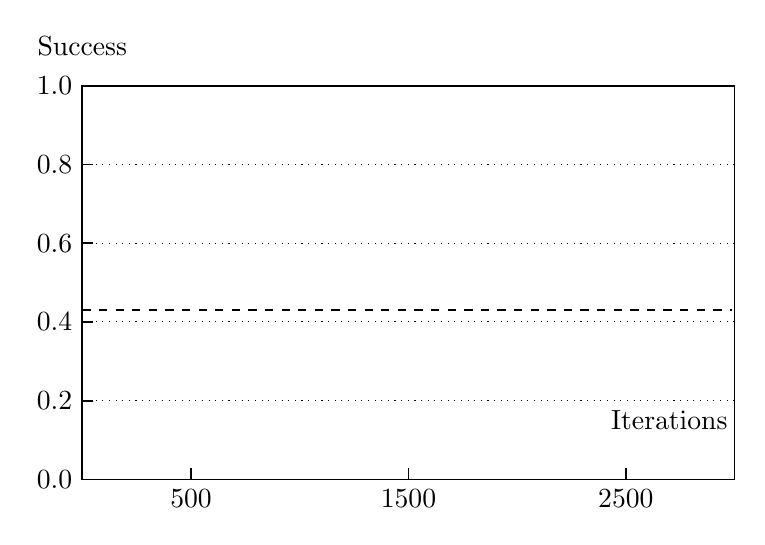
\begin{tikzpicture}[x=0.00276cm,y=5cm]
    % Draw the axes and grid lines
    \draw[-] (0,0) -- (0,1) -- (3000,1) -- (3000,0) -- cycle; 
    \draw[-,thin, dotted, ystep=0.2, xstep=3000] (0,0) grid (3000,1);
    \foreach \x in {500, 1500, 2500}  \draw [-,xshift=0](\x,4pt) -- (\x,-1pt);
    \foreach \y in {0.0,0.2,0.4,0.6,0.8,1.0}  \draw [-,yshift=0](4pt,\y) -- (-1pt,\y);
    \foreach \x/\xtext in {500/500, 1500/1500, 2500/2500} \node at (\x,0) [below] {$\xtext$};
    \foreach \y/\ytext in {0.0,0.2,0.4,0.6,0.8,1.0}  \node at (0,\y) [left] {$\ytext$};
    \node at (0,1.1) {Success};
    \node at (2700,0.15) {Iterations};
    \draw[-,red] plot[mark=x,mark size=4,mark options={color=red}] 
			file {figs/data/test05v3gm.CC.tikzdata};
    \draw[-,thin,densely dashed,black] plot[mark=x,mark size=4,mark options={color=black}] 
			file {figs/data/test05v3gm.CP.tikzdata};
    \draw[-,thin,densely dashed,black] plot[mark=o,mark size=2,mark options={color=black}] 
			file {figs/data/test05v3gm.SP.tikzdata};
    % Also draw the expected convergence: 0.9^8 actions=0.43046
    \draw[dashed,-,yshift=0](0,0.43046) -- (3000,0.43046);

\end{tikzpicture}

\end{center}
\caption{Comparison of the new configurations \BUL+$E'$ (diamonds) and \CL+$E'$ (squares) against the earlier \BUL+$E$ (circles) and \CL+$E$ (triangles) for the \BUL-favouring structure $\T_2$.}
\label{fig:T2_result2}
\end{figure}

We now consider a new structure $\T_4$ that is based on the typical setting (so is not intentionally biased towards one approach), and that has the property that a world $W$ may have two solutions, each in a different sub-tree. Furthermore one solution is always \textit{better} than the other because it has a higher chance of success (in our environment we model this by varying the number of actions required in the solution where each action has a $10\%$ chance of failure). Finally, the structure is crafted so that the likelihood of finding the sub-optimal solution is higher. The purpose is to understand how our approaches behave when optimality is important. Here we expect that the coverage-based exploration of $E'$ should benefit over $E$ in finding the optimal solutions first. 

\begin{figure}[ht]
\begin{center}
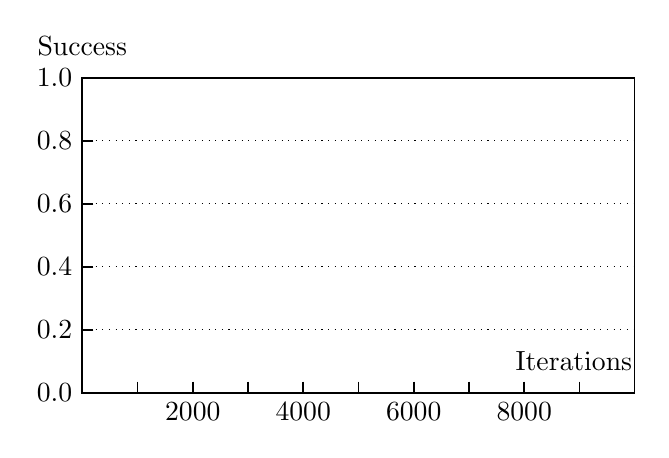
\begin{tikzpicture}[x=0.0007cm,y=4cm]
    % Draw the axes and grid lines
    \draw[-] (0,0) -- (0,1) -- (10000,1) -- (10000,0) -- cycle; 
    \draw[-,thin, dotted, ystep=0.2, xstep=10000] (0,0) grid (10000,1);
    \foreach \x in {0,1000,...,10000}  \draw [-,xshift=0](\x,4pt) -- (\x,-1pt);
    \foreach \y in {0.0,0.2,0.4,0.6,0.8,1.0}  \draw [-,yshift=0](4pt,\y) -- (-1pt,\y);
    \foreach \x/\xtext in {2000/2000, 4000/4000, 6000/6000, 8000/8000} \node at (\x,0) [below] {$\xtext$};
    \foreach \y/\ytext in {0.0,0.2,0.4,0.6,0.8,1.0}  \node at (0,\y) [left] {$\ytext$};
    \node at (0,1.1) {Success};
    \node at (8900,0.1) {Iterations};
    \draw[-] plot[mark=square,mark size=2,mark options={color=black}] 
			file {data/testMultiSolutionsR.CC.tikzdata};
    \draw[-,thin,densely dashed,gray] plot[mark=triangle,gray,mark size=3,mark options={color=gray}] 
			file {data/testMultiSolutionsR.CP.tikzdata};
    \draw[-] plot[mark=diamond,mark size=3,mark options={color=black}] 
			file {data/testMultiSolutionsR.SC.tikzdata};
    \draw[-,thin,densely dashed,gray] plot[mark=o,gray,mark size=2,mark options={color=gray}] 
			file {data/testMultiSolutionsR.SP.tikzdata};

\end{tikzpicture}

\end{center}
\caption{Comparison of all configurations (\BUL+$E'$ (diamonds), \CL+$E'$ (squares), \BUL+$E$ (circles), \CL+$E$ (triangles)) for new structure $\T_4$ with local solutions.}
\label{fig:T4_result}
\end{figure}

Figure \ref{fig:T4_result} shows the results for $\T_4$ where \CL+$E'$ (squares) easily outperforms \CL+$E$ (triangles) and \BUL (diamonds and circles). The reason why the other configurations are sub-optimal is because they do not take into account the structure of the tree and therefore tend to focus exploration in the sub-tree where the first solution was found (which likely is the sub-optimal one in our case) \footnote{Note that \BUL+$E'$ does consider the tree structure but as explained earlier it's behaviour is effectively the same as \BUL+$E$}.


The above results are significant because they highlight a configuration \CL+$E'$ that performs well in \textit{all} proposed structures: the \CL-favouring $\T_1$, the \BUL-favouring $\T_2$, the typical setting $\T_3$, and the typical setting with optimal solutions $\T_4$, making it a good candidate for the general setting. Moreover, the \CL-based configuration is a simpler alternative to the \BUL-based configuration, further adding to it's appeal.

\Omit{
\subsection{Discussion}

In Section \ref{sec:coverage} we presented a \textit{coverage}-based
confidence measure that combined with the \dt classification gives an
informed plan selection function (Equation \ref{eqn:coverage}) that
benefits our context learning approaches \CL\ and \BUL. Now, 
}
Since the
coverage $c_T(S)$ in Equation \ref{eqn:coverage} is simply a
confidence measure, then the way it is \textit{used} will determine
the weighting of the confidence in the final plan selection
probability $p'_T(w)$. For instance we could replace $c_T(S)$ in
Equation \ref{eqn:coverage} with $c_T(S)^{1/b}$ where $b$ is the
weighting (and $b=1$ gives us the original Equation
\ref{eqn:coverage}). Then adjusting $b \rightarrow 0, (0 \ne b < 1$)
we get more \BUL+$E$-like performance, while adjusting $b \rightarrow
\infty (b > 1)$ will result in more \CL+$E$-like performance. In fact,
an improved agent could reference the (static) goal-plan tree
structure at runtime and adjust $b$ automatically based on the offline
compiled knowledge of which approach works better for which tree
topology. 
% This extension is left as a future implementation exercise. 

We noted earlier in Section \ref{sec:experiments} that plan execution
in real systems is often not cost-free, so presumably the agent would
not execute a plan with too low a probability of success. We also show
that such deliberation does not favour \CL\ but does \BUL. It is clear
that choosing not to execute a plan below a threshold probability of
failure would also hurt the \CL+$E'$ configuration (though
not as much as \CL+$E$). For such systems, we suggest that the
weighting $b$ be used to get the preferred \BUL-like performance. 

One critique of the coverage-based confidence measure is that it has a
defined start ($c_T(S)=0$) and end state ($c_T(S)=1$). For a real
system however, learning and re-learning will occur in an endless loop
as the agent continually tries to adapt to a changing
environment. This implies that our confidence in a \dt's
classification would also require calibration based on a changing
environment. If the change in the environment is deliberate (for
instance the agent was moved into a new environment) then the coverage
$c_T(S)$ could be reset and confidence \textit{re-built}. Without such
a signal the agent must rely on measuring per-goal performance in
order to pick up failures that could be attributed to environmental
changes. The problem of identifying changes that warrant new learning
as compared to adapting previous learning, however, is generally
considered to be very difficult.
%a much harder one. 



%%%%%%%%%%%%%%%%%%%%%%%%%%%%%%%%%%%%%%%%%%%%%%%%%%%%
\section{Discussion and Conclusion}\label{sec:discussion}
%%%%%%%%%%%%%%%%%%%%%%%%%%%%%%%%%%%%%%%%%%%%%%%%%%%%

In this paper, we proposed a technique to enhance the typical plan selection
mechanism in BDI systems by allowing agents to learn and adapt the context
conditions of plans in the agent's plan library.
% %
As designing adequate context conditions that take full account of the agent's
environment for its complete life-cycle is an non-trivial task, a framework that
allows for the \emph{refinement} of (initial) context conditions of plans
\textit{based on online experience} is highly desirable.
% %
To this end, we extended the typical BDI programming framework to use \dt{}s as
(part of) plan's context conditions and provided a probabilistic plan selection
mechanism that caters for both exploration and exploitation of plans.
% %
After empirically evaluating different learning strategies suitable for BDI
agents against various kind of plan libraries, we concluded that an aggressive
learning approach combined with plan selection scheme that uses a confidence
measure based on the notion of plan coverage is the best candidate for the
general setting.
% %
The work carried out here is significant for the BDI agent-oriented programming
community, in that it provides a solid foundations for going beyond the standard
static kind of BDI agents.


The framework presented here made a number of simplifying assumptions.
% %
Our experiments did not consider the effects of conflicting interactions between
sub-goals of a plan. In fact, the way a sub-goal is resolved may affect how the
next sub-goal can be addressed or even if it can be resolved at all.
% %
Our current implementation is not possible to detect and learn such interactions;
each subgoal is treated ``locally.'' To handle such interactions, the selection
of a plan for a resolving sub-goal should also be predicated the goals higher
than the sub-goal, that is, it should take into account the ``reasons'' for the
sub-goal.
% %
Similarly, we did not consider the effects of using goal failure recovery, under
which alternative plans for a goal are tried upon the failure of a plan.
% %
Also, we have only dealt with domains described via boolean propositions. To
handle continuous attributes (e.g., discretize \emph{temperature}), our approach
requires that either these attributes are discretized or additional discrete
attributes be used to test the continuous ones (e.g., \emph{cold}, \emph{warm},
and \emph{hot}).
% %
% Lastly, we point out that even though we have used environments with a simple
% stochastic model, our results apply trivially to agents acting in environments
% based on more complex models.


One critique of the coverage-based confidence measure used is that it has a
defined end state, namely $c_T(w)=1$. In a real system, however, learning and
re-learning will occur indefinitely, as the agent continually tries to
\emph{adapt} to a changing environment. This implies that an agent's confidence
in a \dt's classification would also require calibration when the environment has
changed. If the change was deliberate, then our confidence could be reset and
subsequently \textit{re-built}. Without such an explicit signal, the agent must
rely on other methods for determining when the environment has changed
significantly.
% %
An appealing measure for recognising environmental changes is through the
relatedness of its features. For instance, an observation that the grass is
\textit{wet} may have a high correlation to the fact that it is \textit{raining}.
If at some point, the agent were to witness a world where it is not raining but
the grass is indeed wet (for some other new reasons), then this world would be
``atypical,''  and as a result, the agent may have reason to reduce its
confidence in a plan's \dt\ classification of this new world.
% %
It turns out that efficient algorithms exist---some already included in the
\weka\ library---that perform inference in and learning of Bayesian networks
\cite{Mitchell97:ML}, which the agent can appeal to build a model of the
environment for the purposes just described.



The issue of combining learning and deliberative approaches for decision making
in autonomous systems has not been widely addressed.
% %
In~\cite{Riedmiller01}, learning is used \emph{prior to deployment} for acquiring
low level robot soccer skills that are then treated as fixed methods in the
deliberative decision making process once deployed.
% %
Hern\'andez et al. \cite{Hernandez04:Learning} give a preliminary account of how
decision trees may be induced on plan failures in order to find an alternative
logical context conditions in a deterministic paint-world example.
% %
More recently, \cite{Zhuo09:Learning} proposes a method for learning hierarchical
task network (HTN) method preconditions under partial observations. There, a set
of  constraints are constructed from observed decomposition trees that are then
solved \emph{offline} using a constraint solver. Despite HTN systems being
automated planning frameworks, rather than execution frameworks, these are highly
related to BDI agent systems when it comes to the \emph{know-how} information
used---learning methods' preconditions amounts to learning plan's context
conditions.
% %
In constrast, in our work, learning and deliberation are fully integrated in a
way that one impacts the other and the classical exploration/exploitation dilemma
applies.
% Initially, instead of following a random exploration policy (as is the case for
% agents with no initial knowledge), our agents are guided by the existing domain
% knowledge inherent in the BDI hierarchy.





%%%%%%%%%%%%%%%%%%%%%%%%%%%%%%%%%%%%%%%%%%%%%%%%%%%%


%ACKNOWLEDGMENTS are optional
%\section{Acknowledgments}
%This section is optional

%
% The following two commands are all you need in the
% initial runs of your .tex file to
% produce the bibliography for the citations in your paper.
% \bibliographystyle{abbrv}
% \bibliography{aamas10bdilearning}

\small

\begin{thebibliography}{10}

\medskip

\bibitem{Airiau:IJAT09}
S.~Airiau, L.~Padgham, S.~Sardina, and S.~Sen.
\newblock Enhancing Adaptation in {BDI} Agents Using Learning Techniques.
\newblock In {\em Intr. Journal of Agent Technologies and Systems}, 2009.

%\bibitem{APSS08}
%S.~Airiau, L.~Padham, S.~Sardina, and S.~Sen.
%\newblock Enhancing adaptation in {BDI} agents using learning techniques.
%\newblock {\em International Journal of Agent Technologies and Systems
%  (IJATS)}, 1(2):1--18, Jan. 2009.

\bibitem{Benfield:AAMAS06}
S.~S. Benfield, J.~Hendrickson, and D.~Galanti.
\newblock Making a strong business case for multiagent technology.
\newblock In {\em Proc. of AAMAS}, pages 10--15. ACM Press, 2006.

\bibitem{jasonbook}
R.~Bordini, J.~H{\"u}bner, and M.~Wooldridge.
\newblock {\em Programming Multi-agent Systems in {AgentSpeak} Using {Jason}}.
\newblock Wiley Series in Agent Technology. Wiley, 2007.

\bibitem{Bratman88}
M.~Bratman, D.~Israel, and M.~Pollack.
\newblock Plans and resource-bounded practical reasoning.
\newblock {\em Computational Intelligence}, 4(4):349--355, 1988.

\bibitem{Busetta99jack}
P.~Busetta, R.~R{\"o}nnquist, A.~Hodgson, and A.~Lucas.
\newblock {JACK} {I}ntelligent {A}gents: {C}omponents for intelligent agents in
  {J}ava.
\newblock {\em AgentLink News}, 2:2--5, 1999.

\bibitem{Dastani:JAAMAS08-2APL}
M.~Dastani.
\newblock {2APL}: a practical agent programming language.
\newblock {\em Autonomous Agents and Multi-Agent Systems}, 16(3):214--248, 
  2008.

\bibitem{Georgeff89-PRS}
M.~P. Georgeff and F.~F. Ingrand.
\newblock Decision making in an embedded reasoning system.
\newblock In {\em Proc. of IJCAI}, pages 972--978, 1989.

\bibitem{Hernandez04:Learning}
A.~Guerra-Hern\'andez, A.~E. Fallah-Seghrouchni, and H.~Soldano.
\newblock {\em Learning in {BDI} Multi-agent Systems}, volume 3259 of {\em
  LNCS}, pages 218--233.
\newblock Springer, 2004.

\bibitem{Hindriks99:Agent}
K.~Hindriks, F.~D. Boer, W.~V.~D. Hoek, and J.~Meyer.
\newblock Agent programming in {3APL}.
\newblock {\em Autonomous Agents and Multi-Agent Systems}, 2(4):357--401, 1999.

\bibitem{Mitchell97:ML}
T.~Mitchell.
\newblock {\em Machine Learning}.
\newblock McGraw Hill, 1997.

\bibitem{MorelyM:AAMAS04-SPARK}
D.~Morley and K.~L. Myers.
\newblock The {SPARK} agent framework.
\newblock In {\em Proc. of AAMAS}, pages 712--719, 2004.

\bibitem{Pollack92-IRMA}
M.~E. Pollack.
\newblock The uses of plans.
\newblock {\em Artificial Intelligence Journal}, 57(1):43--68, 1992.

\bibitem{Riedmiller01}
M.~Riedmiller, A.~Merke, D.~Meier, A.~Hoffman, A.~Sinner, O.~Thate, and
  R.~Ehrmann.
\newblock Karlsruhe brainstormers - a reinforcement learning approach to
  robotic soccer.
\newblock In {\em {RoboCup} 2000: Robot Soccer World Cup {IV}}, 2001.

\bibitem{Swere06:Fast}
E.~Swere, D.~Mulvaney, and I.~Sillitoe.
\newblock A fast memory-efficient incremental decision tree algorithm and its
  application to mobile robot navigation.
\newblock In {\em Proc. of IROS}, 2006.

\bibitem{Thangarajah02}
J.~Thangarajah, M.~Winikoff, L.~Padgham, and K.~Fischer.
\newblock Avoiding resource conflicts in intelligent agents.
\newblock In {\em Proc. of ECAI}, pages 18--22, 2002.

\bibitem{Utgoff97Decision}
P.~E. Utgoff, N.~C. Berkman, and J.~A. Clouse.
\newblock Decision tree induction based on efficient tree restructuring.
\newblock {\em Machine Learning}, 29(1):5--44, 1997.

\bibitem{weka99}
I.~Witten and E.~Frank.
\newblock {\em Data Mining: {P}ractical Machine Learning Tools and Techniques
  with Java Implementations}.
\newblock {Morgan Kaufmann}, 1999.

\bibitem{Zhuo09:Learning}
H.~Zhuo, D.~Hu, C.~Hogg, Q.~Yang, and H.~Munoz-Avila.
\newblock {Learning HTN Method Preconditions and Action Models from partial
  Observations}.
\newblock In {\em Proc. of IJCAI}, 2009.

\end{thebibliography}




% You must have a proper ".bib" file
%  and remember to run:
% latex bibtex latex latex
% to resolve all references
%
% ACM needs 'a single self-contained file'!
%

%APPENDICES are optional
%\balancecolumns
%\appendix
%Appendix A
%\section{Headings in Appendices}

\end{document}
